The VBF \Hbb analysis unblinding proceeds in two steps. First, overall strategy is validated with a fit to the $Z$ contribution in a sideband only fit while the Higgs mass window is kept unblinded, described in Section~\ref{sec:vbf-zunblind}.  Then a simultaneous fit to the signal, correlated over all signal regions, and the $Z$ signal, uncorrelated across signal regions, is done over the entire mass region, as described in~\ref{sec:vbf-higgsunblind}. As an alternative interpretation of this analysis the $\mu_{VBF}$ strength is extracted by only allowing $VBF$ events to float in the fit and fixing all other Higgs processes, i.e. ggF, ttH and VH, to Standard Model expectation, as described in~\ref{sec:vbf-higgsunblindvbf}. The combination of inclusive $VBF$ and $VBF+\gamma$ results are presented in~\ref{sec:vbf-higgscomb}.


\subsection{Unblinding of \zjets{} in mass sidebands}
\label{sec:vbf-zunblind}

The fit strategy is first validated in data with a closure obtained in \zjets{} mass sideband fit. We performed a side-band only fit to extract the \zjets{} contribution independently in all regions. The fitted \zjets{} strengths are summarized in Table~\ref{tab:zsidebandfit}, presented with with all experimental and statistical uncertainties.   Note that we have no BDT shape uncertainties on the \zjets{} MC so cannot draw any conclusions from the compatibility of $\mu_Z$ with 1 in the different BDT regions. The effective $\mu_{Z}^{\rm eff}$ of all regions combined is defined as
\begin{equation}
\label{eqn:zsig}
\mu_{Z}^{\rm eff} = \sum \mu_{Z,i}\frac{n_{Z,i}}{\sum n_{Z,i}} 
\end{equation}
where $n_{Z,i}$ is the number of $Z$ events in region $i$, and $\mu_{Z,i}$ is the measured $\mu_Z$ in region $i$.  $\mu_{Z}^{\rm eff}$ is measured to be $1.0\pm 0.4$ in the sideband only fit with a compatibility of $\chi^2/nodf = 5.51/6=0.92$ ($\chi^2$ probability of 48\%).


\begin{table}[htbp]
\centering
\caption{Floating Z normalization parameters in data sideband fit including all systematic uncertainties.}
\label{tab:zsidebandfit}
\begin{tabular}{|l|c|c|}
\hline
Channel      & $\mu_{Z}$   & $\chi^2/ndof$ \\ \hline
2 cen SR I   & 2.6 $\pm$1.3  & 1.1          \\ \hline
2 cen SR II  & 0.4$\pm$0.8  & 0.7          \\ \hline
4 cen SR I   & 2.2$\pm$2.0  & 0.8          \\ \hline
4 cen SR II  & 2.0$\pm$1.9  & 0.9          \\ \hline
4 cen SR III & 1.9$\pm$0.6  & 0.9          \\ \hline
4 cen SR IV  & 0.6$\pm$0.6  & 0.9          \\ \hline
\end{tabular}
\end{table}



%\begin{figure}[htbp]
%  \centering
% 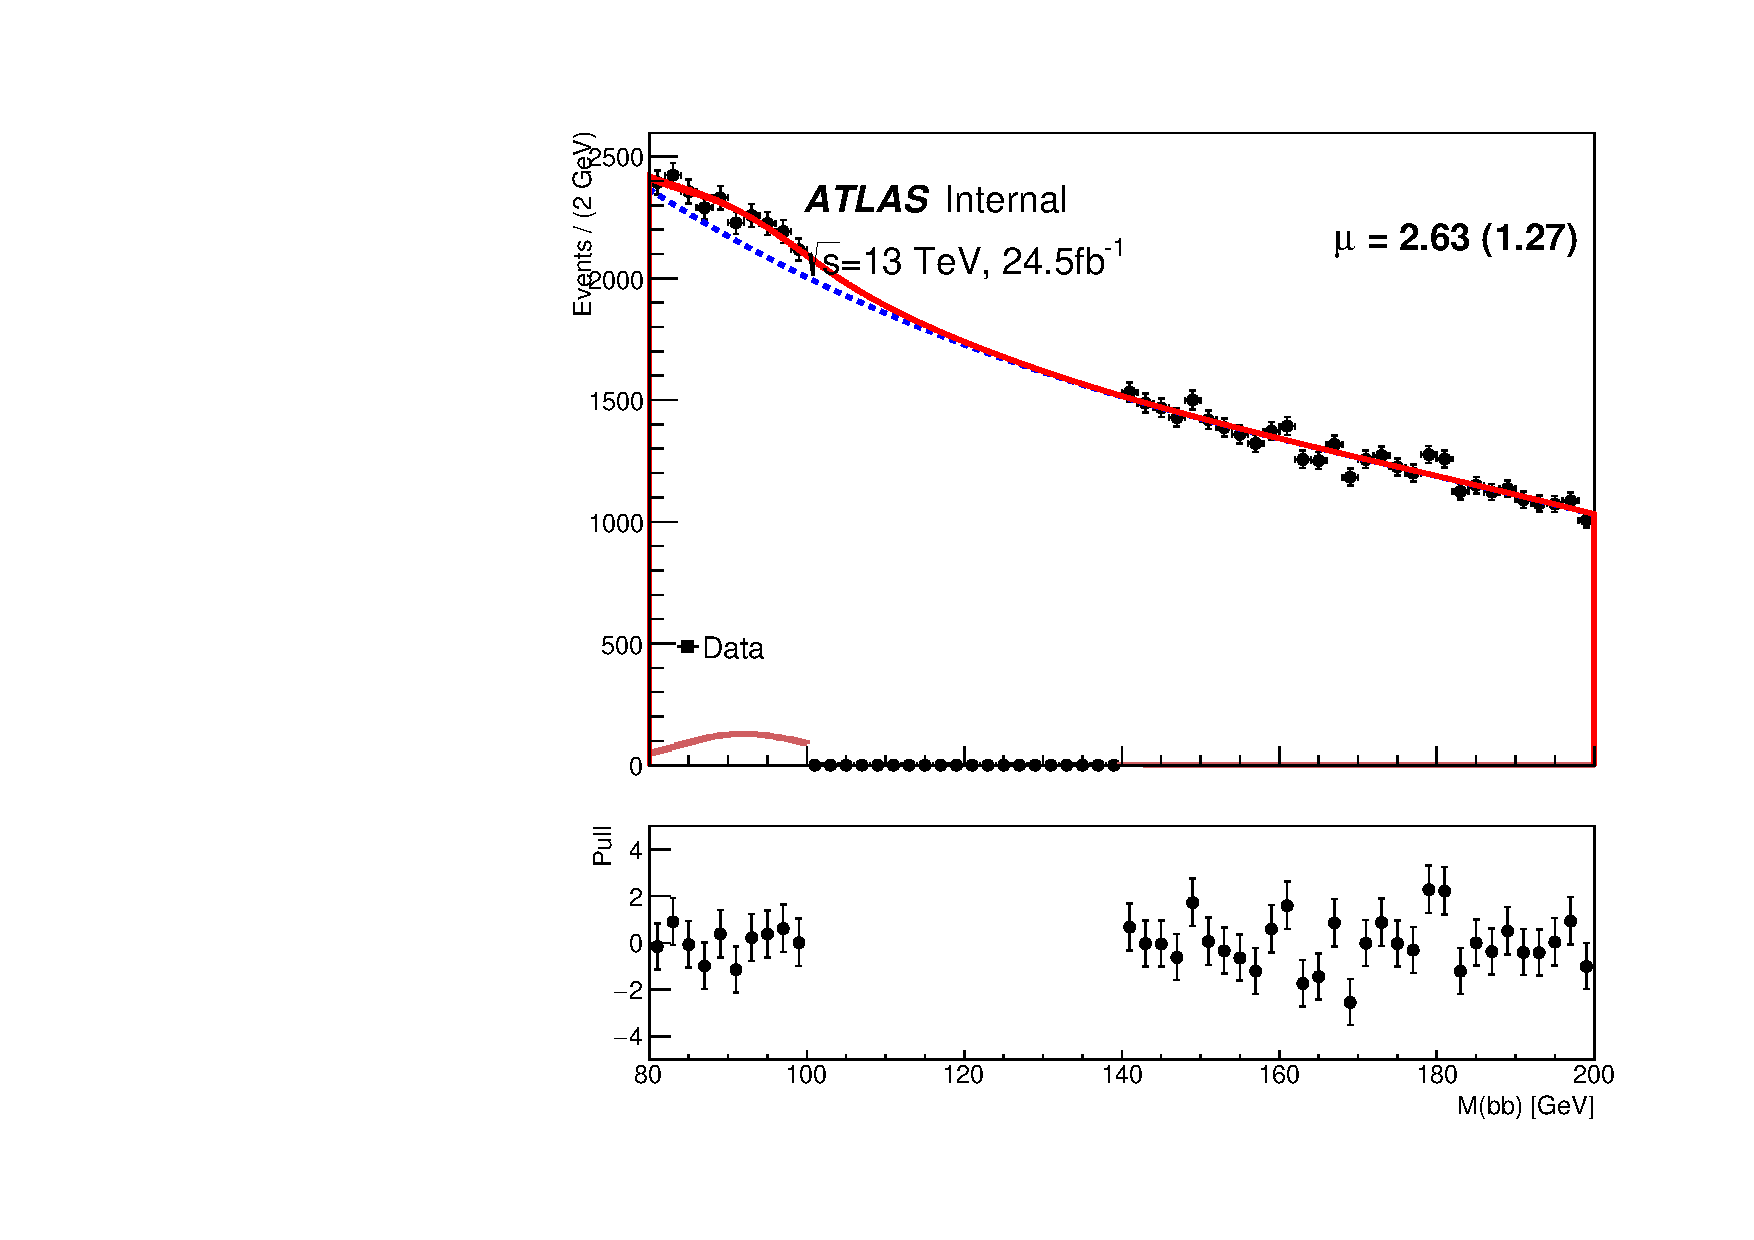
\includegraphics[width=0.24\textwidth]{figures/VBF/zunblind_testVBF_ICHEP_2cen_SRI.pdf}
% 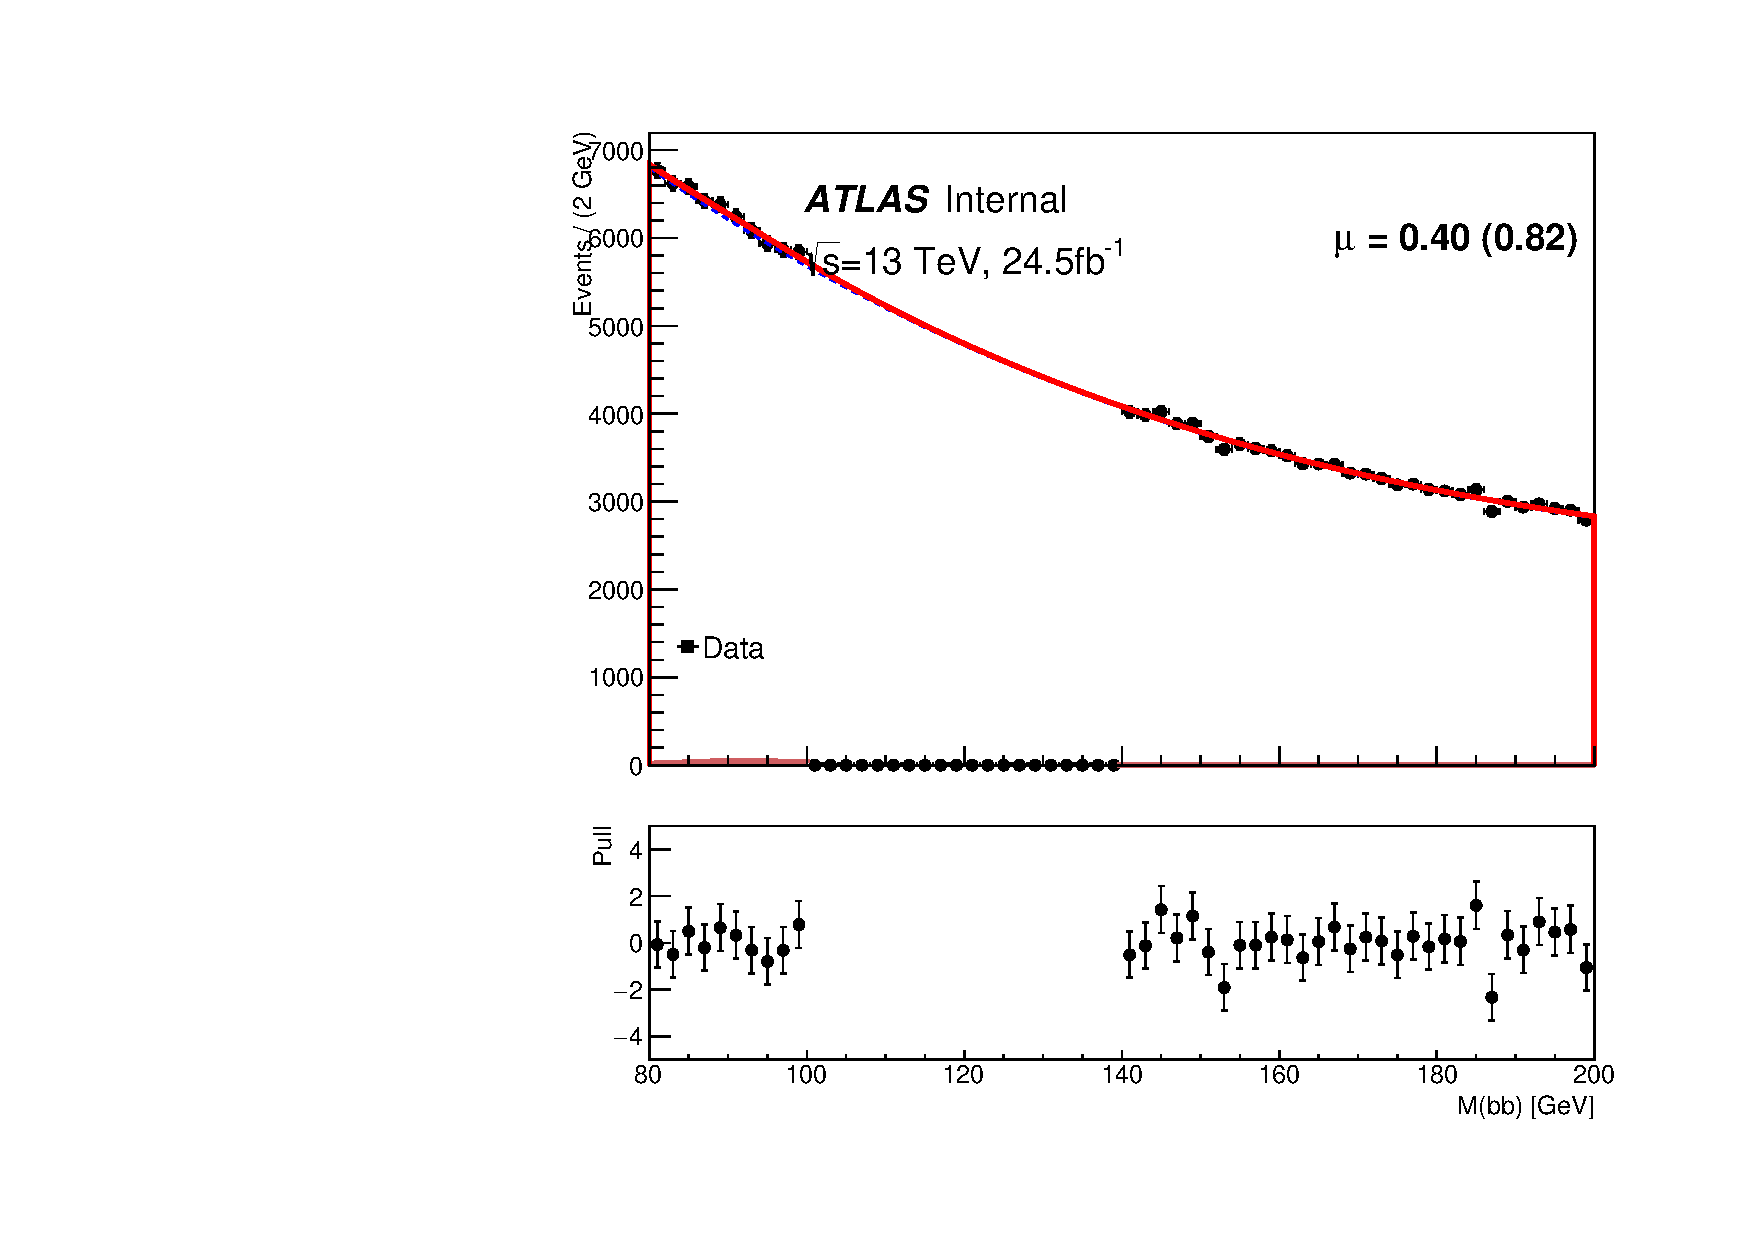
\includegraphics[width=0.24\textwidth]{figures/VBF/zunblind_testVBF_ICHEP_2cen_SRII.pdf}\\
% 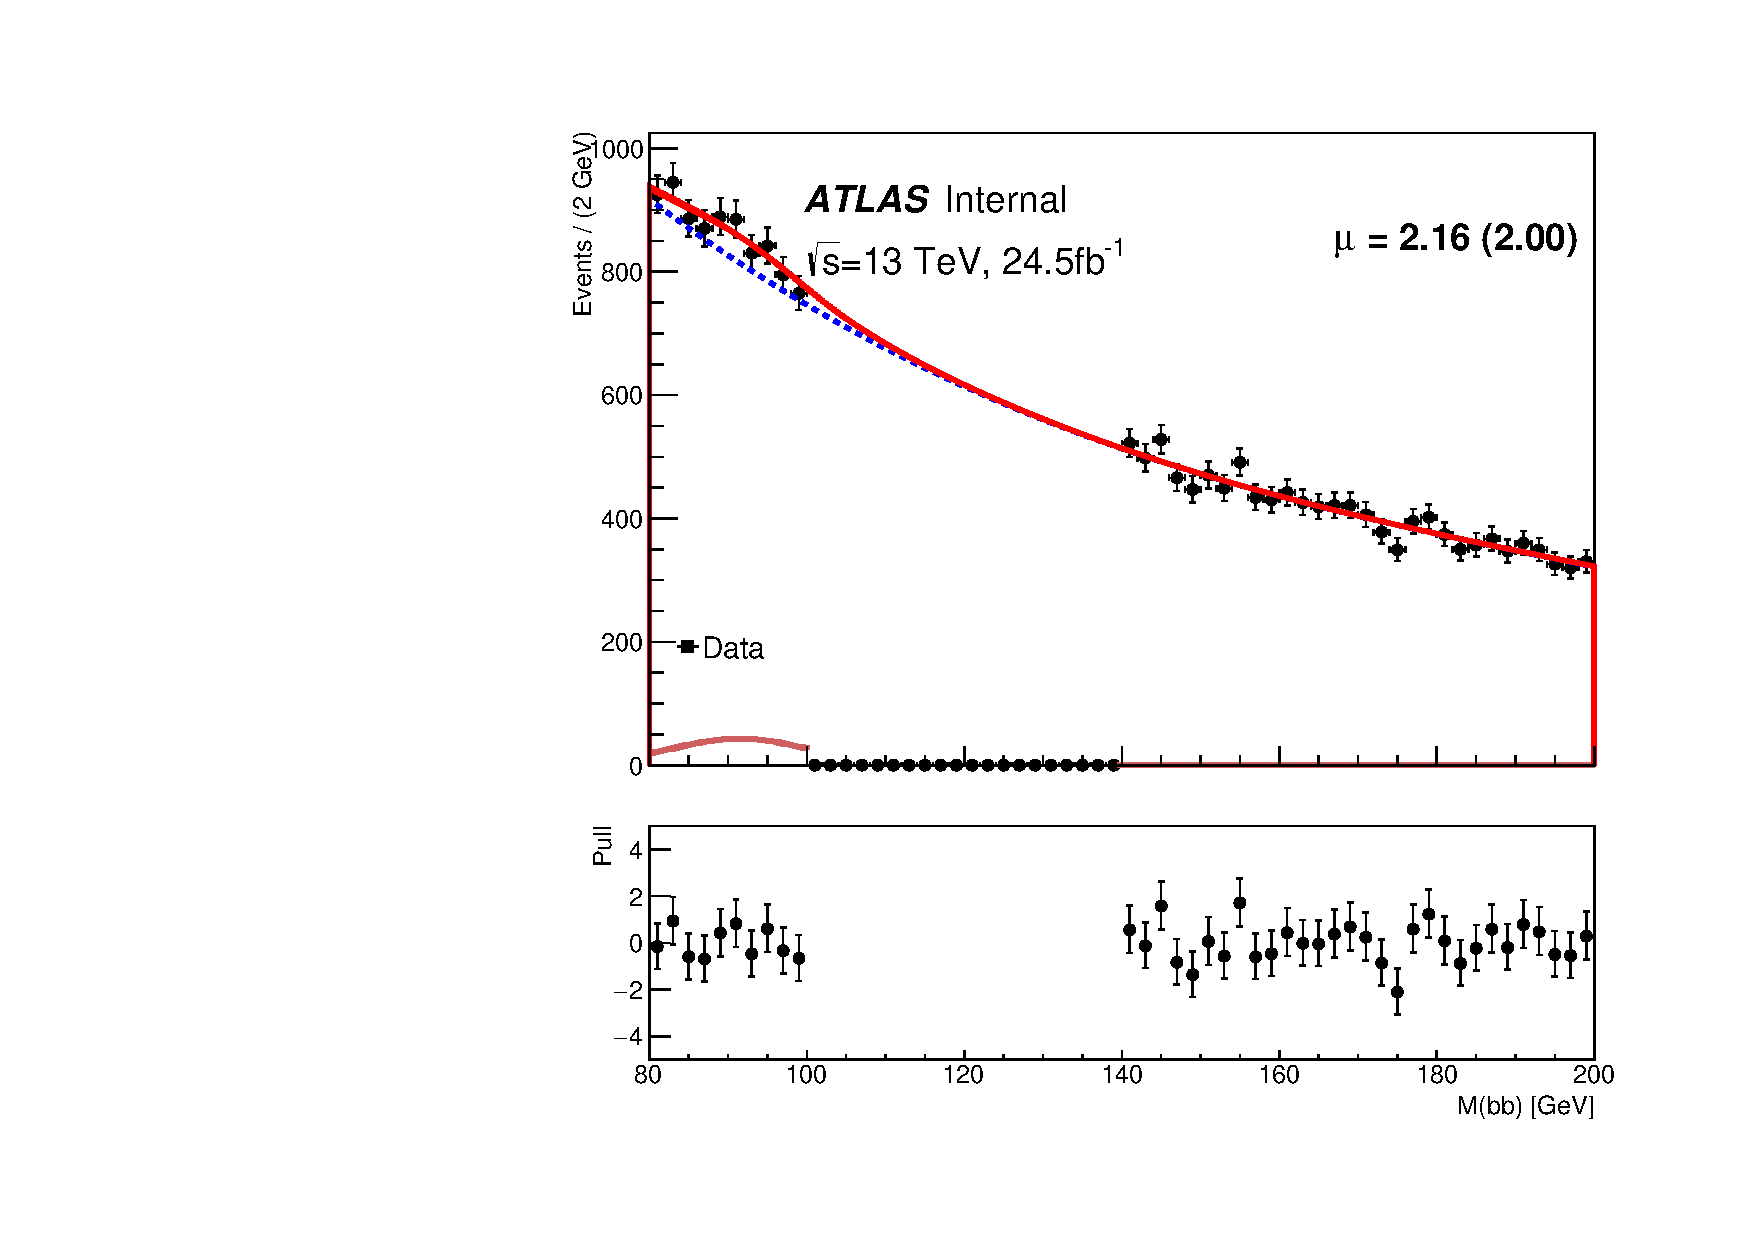
\includegraphics[width=0.24\textwidth]{figures/VBF/zunblind_testVBF_ICHEP_4cen_SRI.pdf}
% 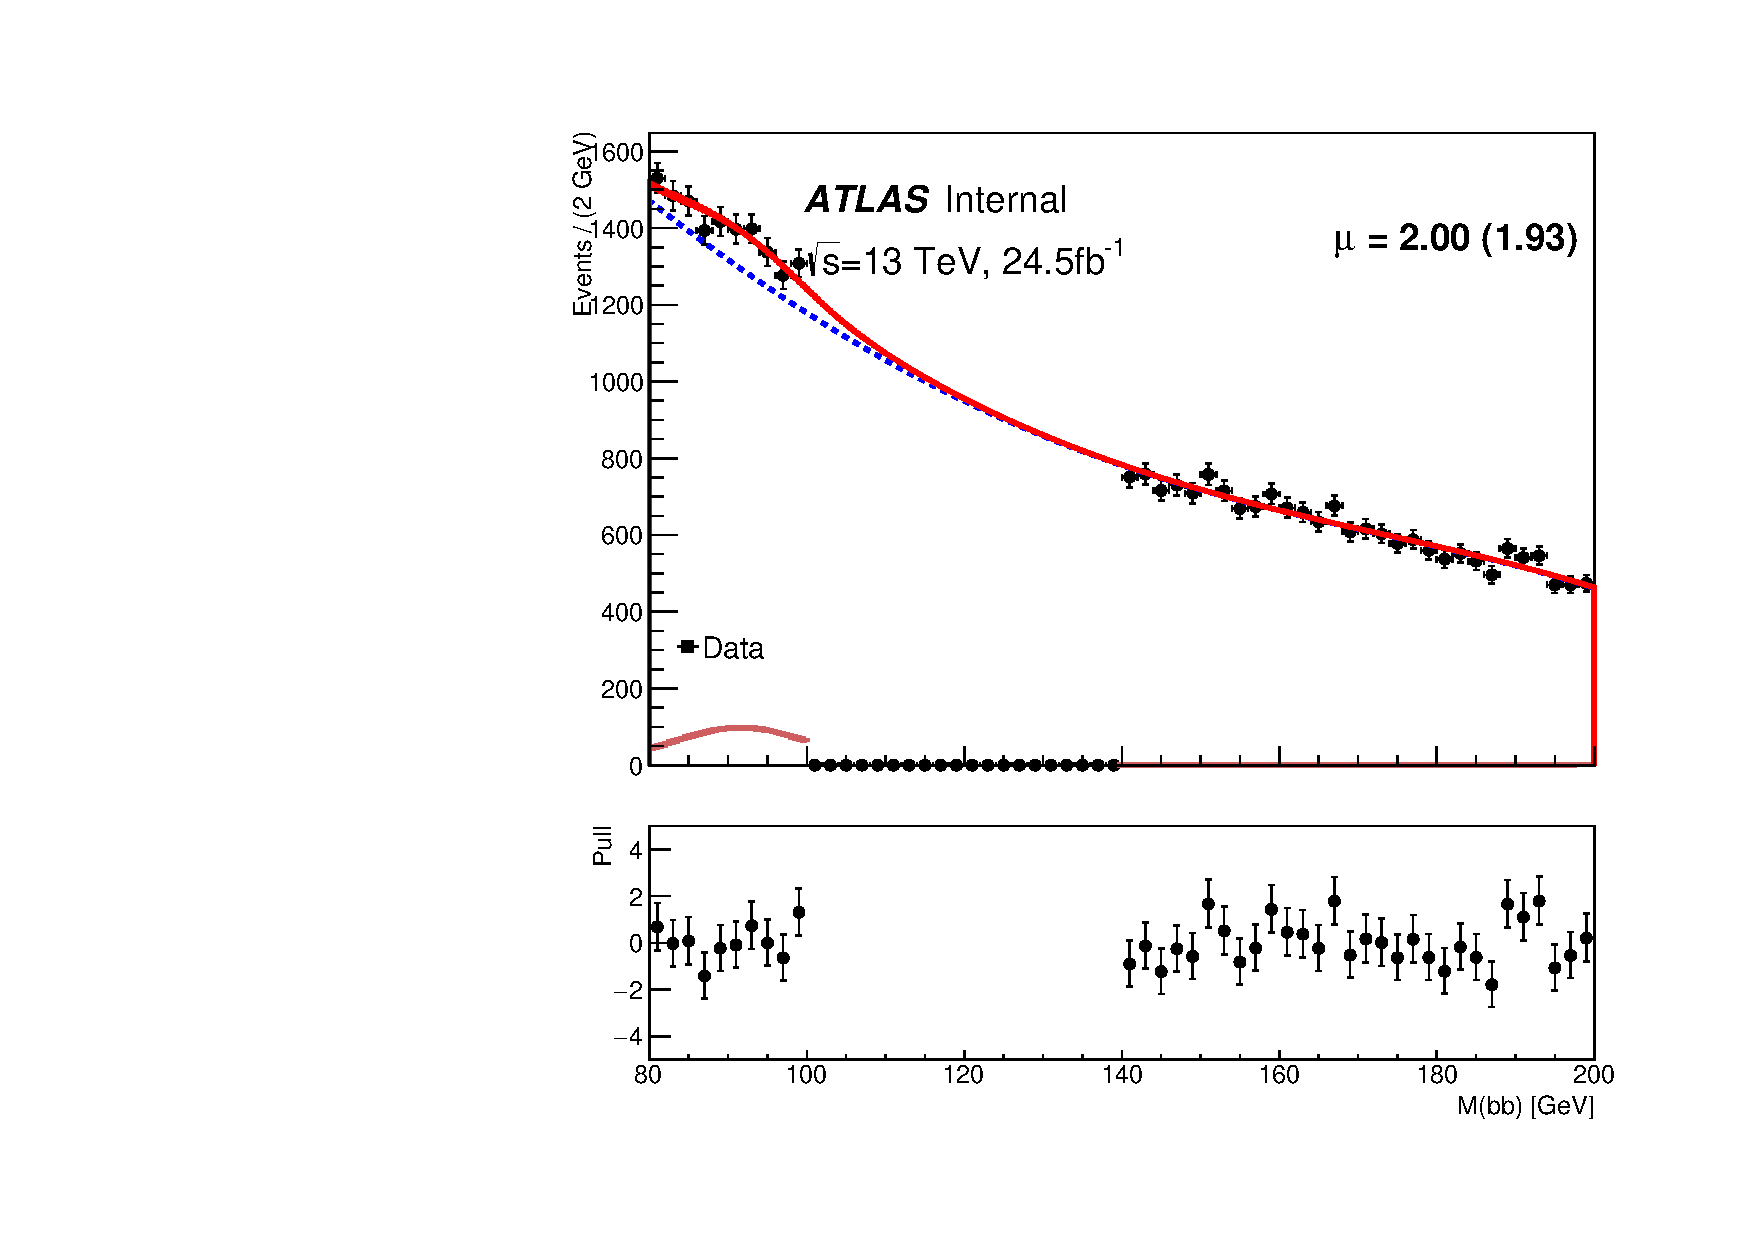
\includegraphics[width=0.24\textwidth]{figures/VBF/zunblind_testVBF_ICHEP_4cen_SRII.pdf}
% 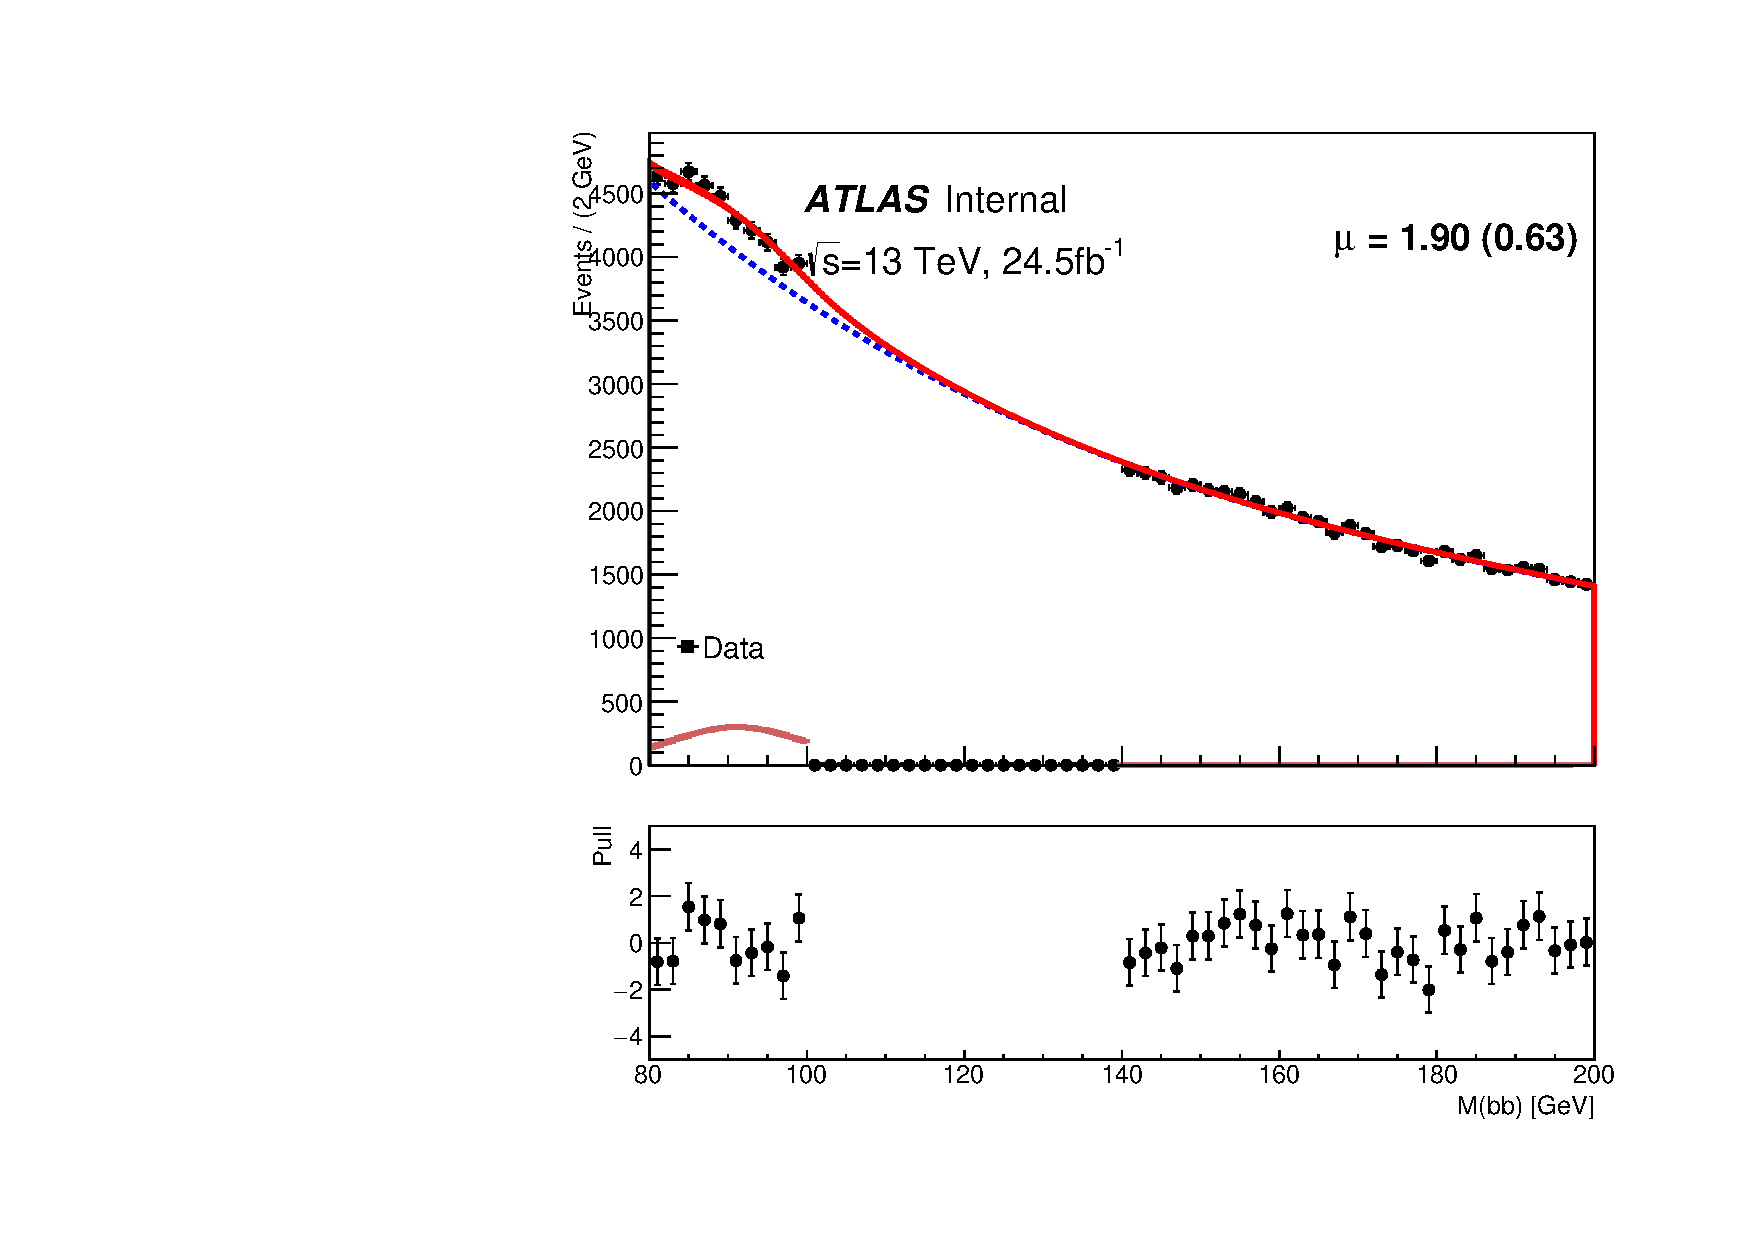
\includegraphics[width=0.24\textwidth]{figures/VBF/zunblind_testVBF_ICHEP_4cen_SRIII.pdf}
% 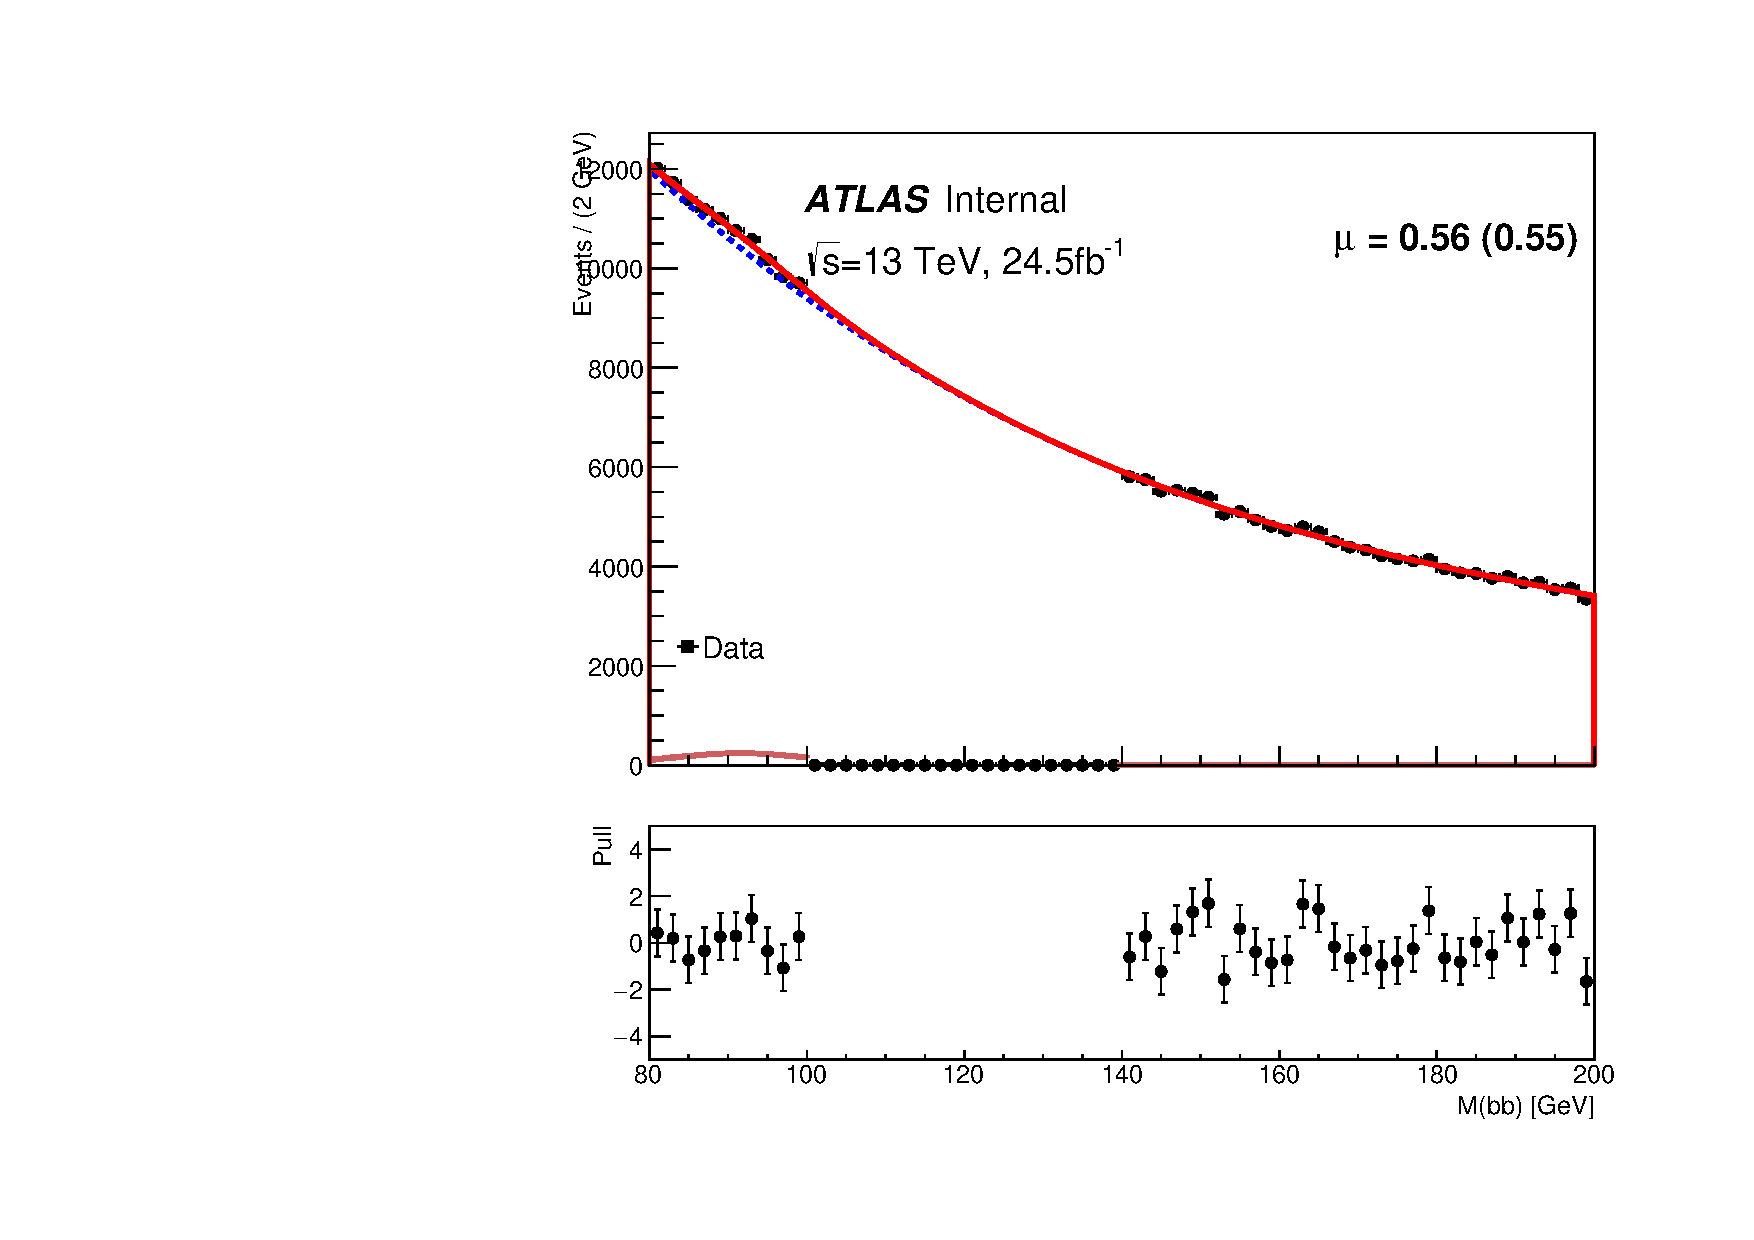
\includegraphics[width=0.24\textwidth]{figures/VBF/zunblind_testVBF_ICHEP_4cen_SRIV.pdf}\\
%\caption{Data and fit model comparison for sideband only \zjets{} fit in \twocentral (top) and \fourcentral channel (bottom) for SR I (left) to SR IV (right).  The data are the black points and the fit model (red), which comprises the continuum background (blue dashed line) and the Z contribution (light red histogram).}
%  \label{fig:vbf-zsidebandfit}
%\end{figure}


\subsection{Extraction of $\mu_{H}$}
\label{sec:vbf-higgsunblind}

The observed value of the Higgs signal strength is $2.7^{+2.2}_{-2.0}$, while the Asimov fit yields $\mu_{H}=1\pm 1.9$. The breakdown of the uncertainty is $\mu_H=2.7^{+1.9}_{-1.9}\textnormal{(stat)}^{+1.1}_{-0.6}\textnormal{(syst)}$ treating the NPs for the analytical background parameterization and normalization as well as the normalization of $Z$ contribution as statistical uncertainty.

%Figures~\ref{fig:vbf-higgsfit_2cen} and ~\ref{fig:vbf-higgsfit_4cen} show the resulting distributions for the \twocentral and \fourcentral channels. %displaying the residuals with respect to the continuum background fit on the bottom panel. % whereas Figures~\ref{fig:vbf-higgsfit_2cen_pull} and~\ref{fig:vbf-higgsfit_4cen_pull} show the pull values with respect to the full background model.  

%The pull values are shown in Figure~\ref{fig:vbf-higgsfitpull} for nuisance parameters with a post-fit impact of more than 4\%.  None of the nuisance parameters are strongly pulled. The largest uncertainty on $\mu_H$ comes from the theory uncertainty on the QCD scale, followed by the background parameterization and the jet energy resolution. The increase of the total uncertainty with respect to the expected value comes from the larger than expected background normalization as well as an increase of the signal systematics which scales as the size of the $\mu_H$. 

The fitted $Z$ values are shown in Table~\ref{tab:zfullfit} for each SR.  Reductions of 30--60\% of the $\mu_Z$ uncertainties are observed with respect to the sideband only fit.  We note again that without BDT shape uncertainties for the $Z$ MC signal, we cannot make any statements about the compatibility of the $Z$ fits with the MC predictions.  A statistical combination of all the channels, as described in Equation~\ref{eqn:zsig}, yields an effective $\mu_Z = 1.2 \pm 0.2$ with a combined $\chi^2/$ndof of 1.05 with a probability of 38.8\%.  

\begin{table}[htbp]
\centering
\caption{Floating Z normalization parameters in full mass range fit.}
\label{tab:zfullfit}
\begin{tabular}{|l|c|c|}
\hline
Channel      & $\mu_{Z}$   & $\chi^2/ndof$ \\ \hline
2 cen SR I   & 2.2$\pm$0.7  & 0.9      \\ \hline
2 cen SR II  & 0.4$\pm$0.4  & 0.7        \\ \hline
4 cen SR I   & 0.3$\pm$1.1  & 0.7         \\ \hline
4 cen SR II  & 1.2$\pm$0.6  & 0.7        \\ \hline
4 cen SR III & 1.4$\pm$0.4  & 0.7         \\ \hline
4 cen SR IV  & 0.9$\pm$0.2  & 0.8          \\ \hline
\end{tabular}
\end{table}


%\begin{figure}[htbp]
%  \centering
% 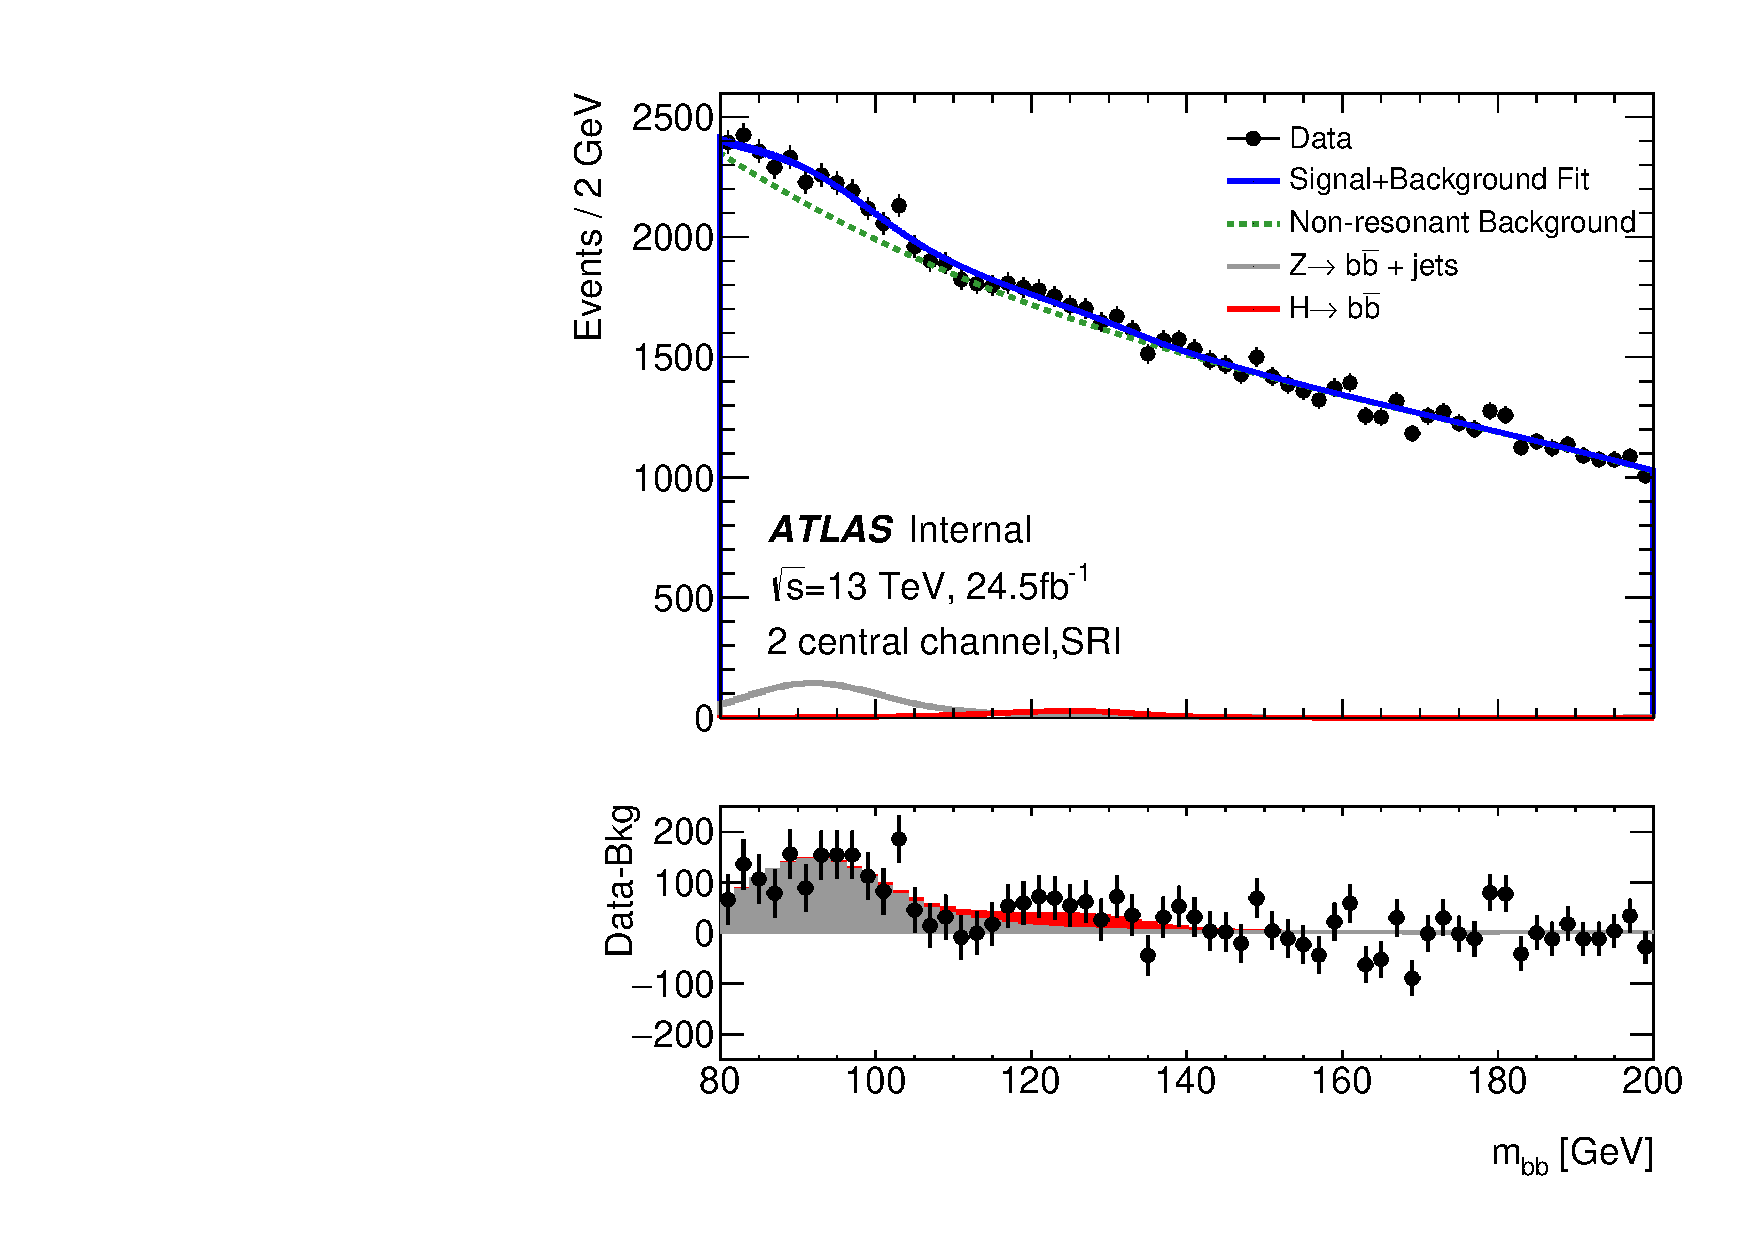
\includegraphics[width=0.48\textwidth]{figures/VBF/unblind_testVBF_ICHEP_2cen_SRI.pdf}
% 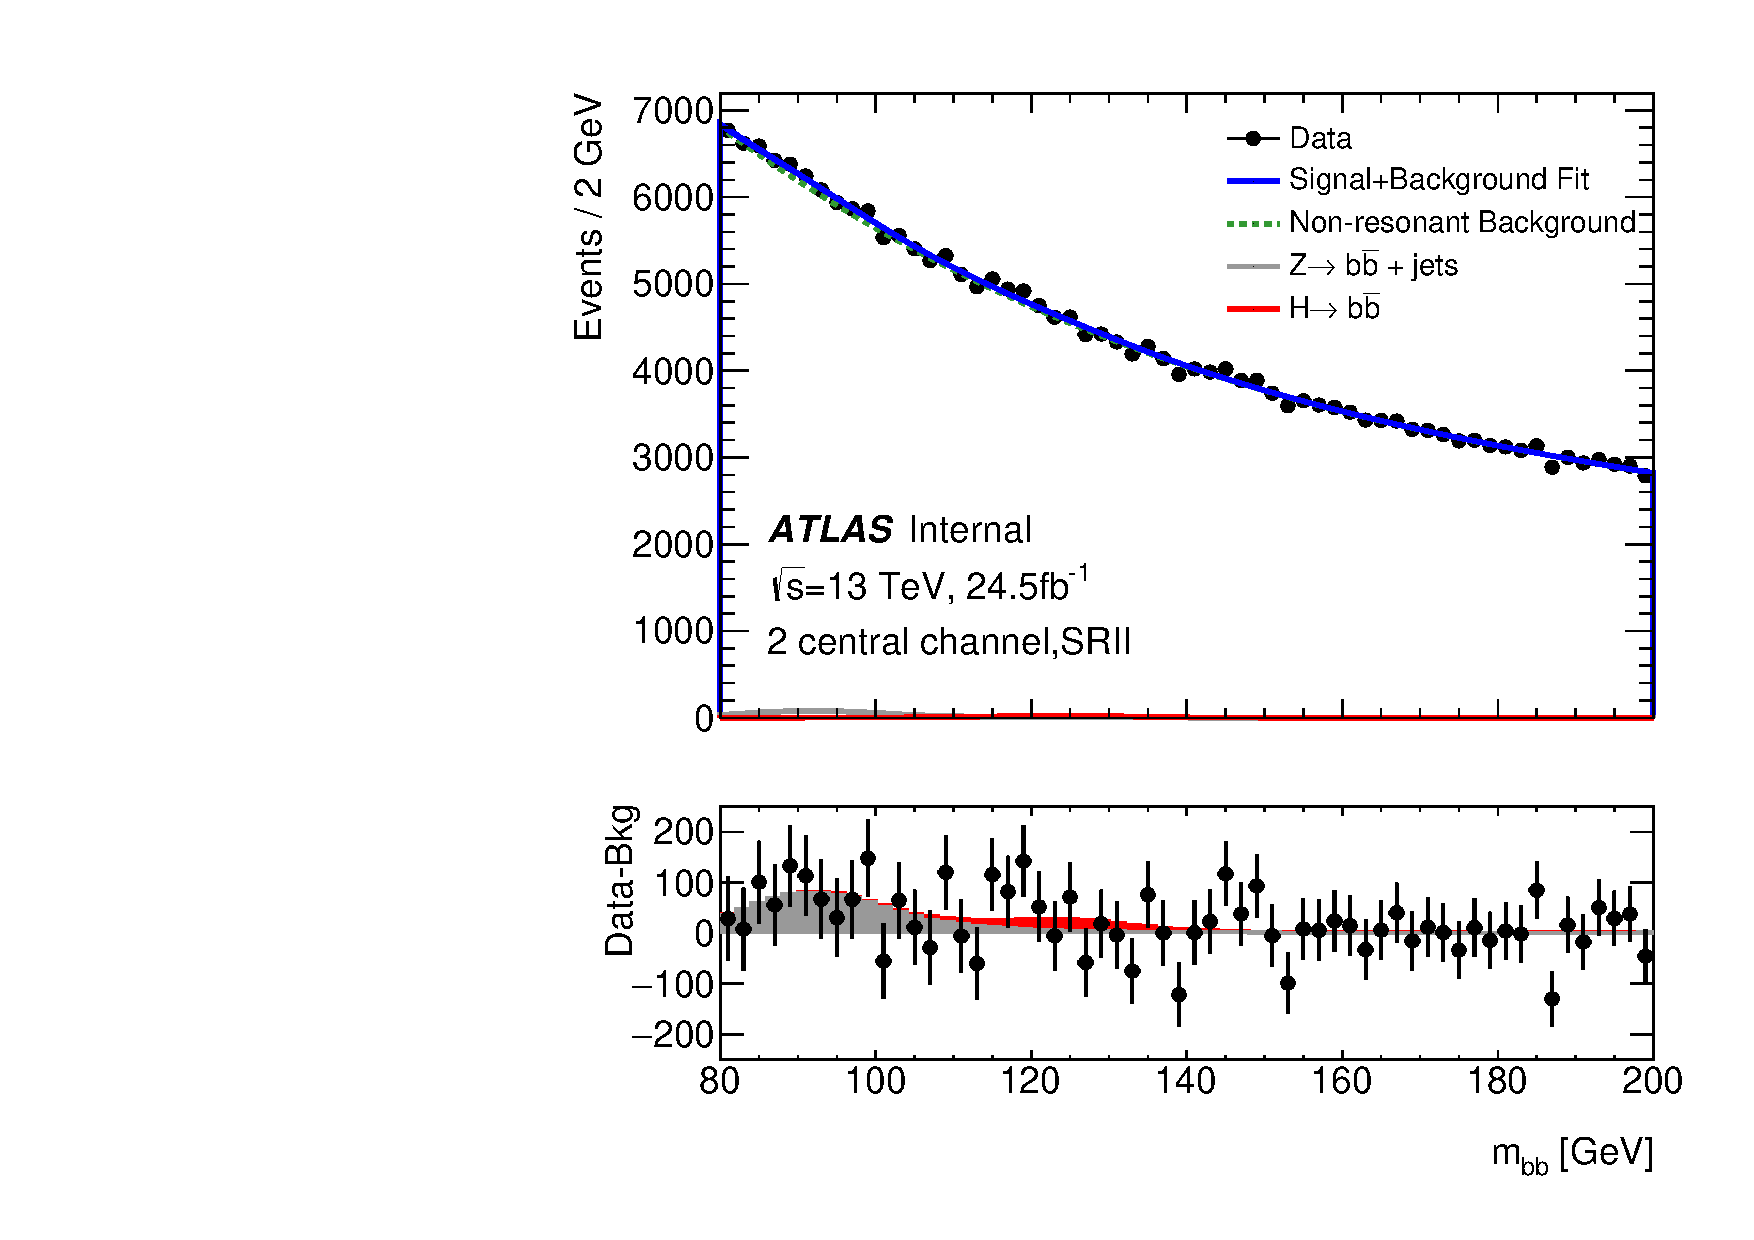
\includegraphics[width=0.48\textwidth]{figures/VBF/unblind_testVBF_ICHEP_2cen_SRII.pdf}\\
%\caption{Data and fit model comparison for profile likelihood fit in the \twocentral channel signal regions.  The fitted continuum background is shown with at  dashed green line, the fitted $Z$ signal in green, and the fitted Higgs signal in red.  The total fit is displayed as the blue line.  The bottom panels show the residual of the data with respect to the continuum background fit, and the fitted $Z$ signal (grey) and Higgs signal (red) are also displayed. }
%  \label{fig:vbf-higgsfit_2cen}
%\end{figure}
%
%\begin{figure}[htbp]
%  \centering
% 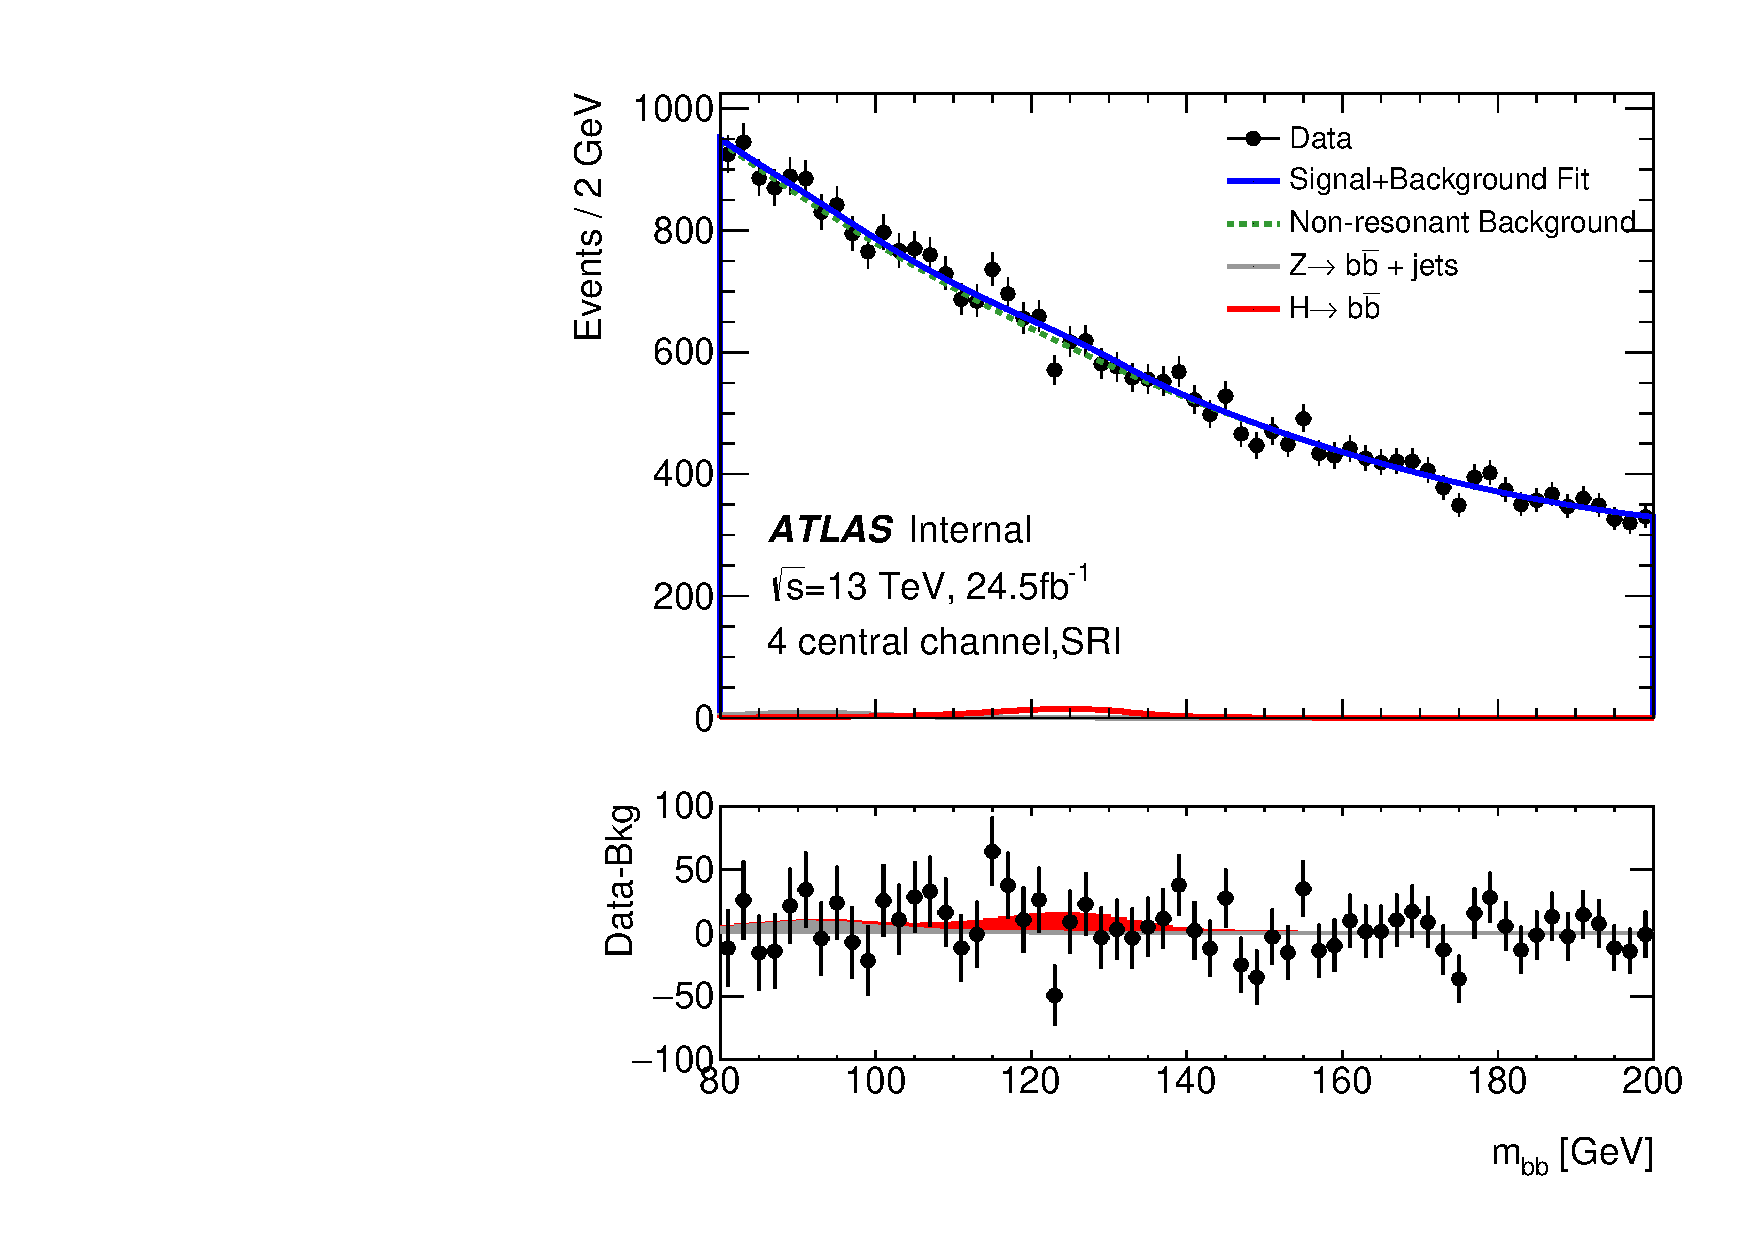
\includegraphics[width=0.48\textwidth]{figures/VBF/unblind_testVBF_ICHEP_4cen_SRI.pdf}
% 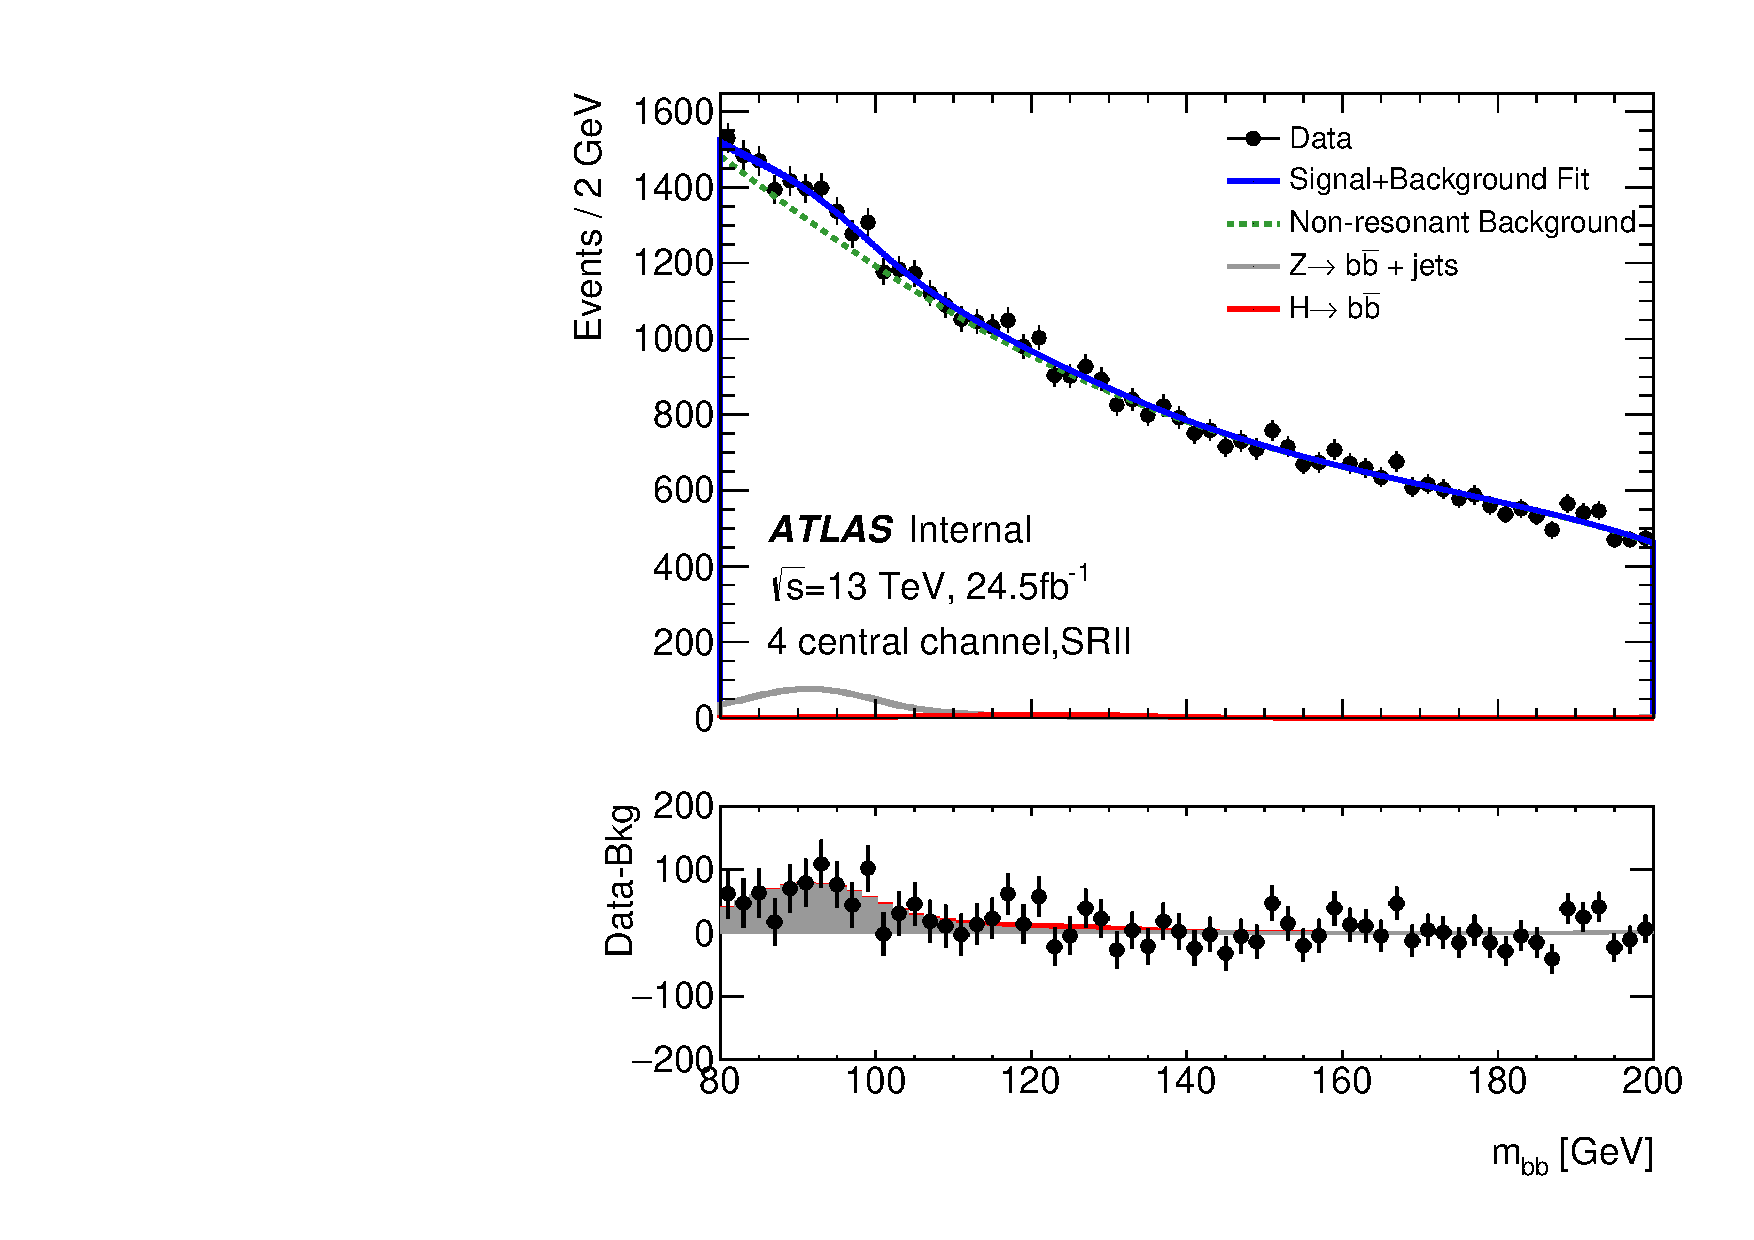
\includegraphics[width=0.48\textwidth]{figures/VBF/unblind_testVBF_ICHEP_4cen_SRII.pdf}\\
% 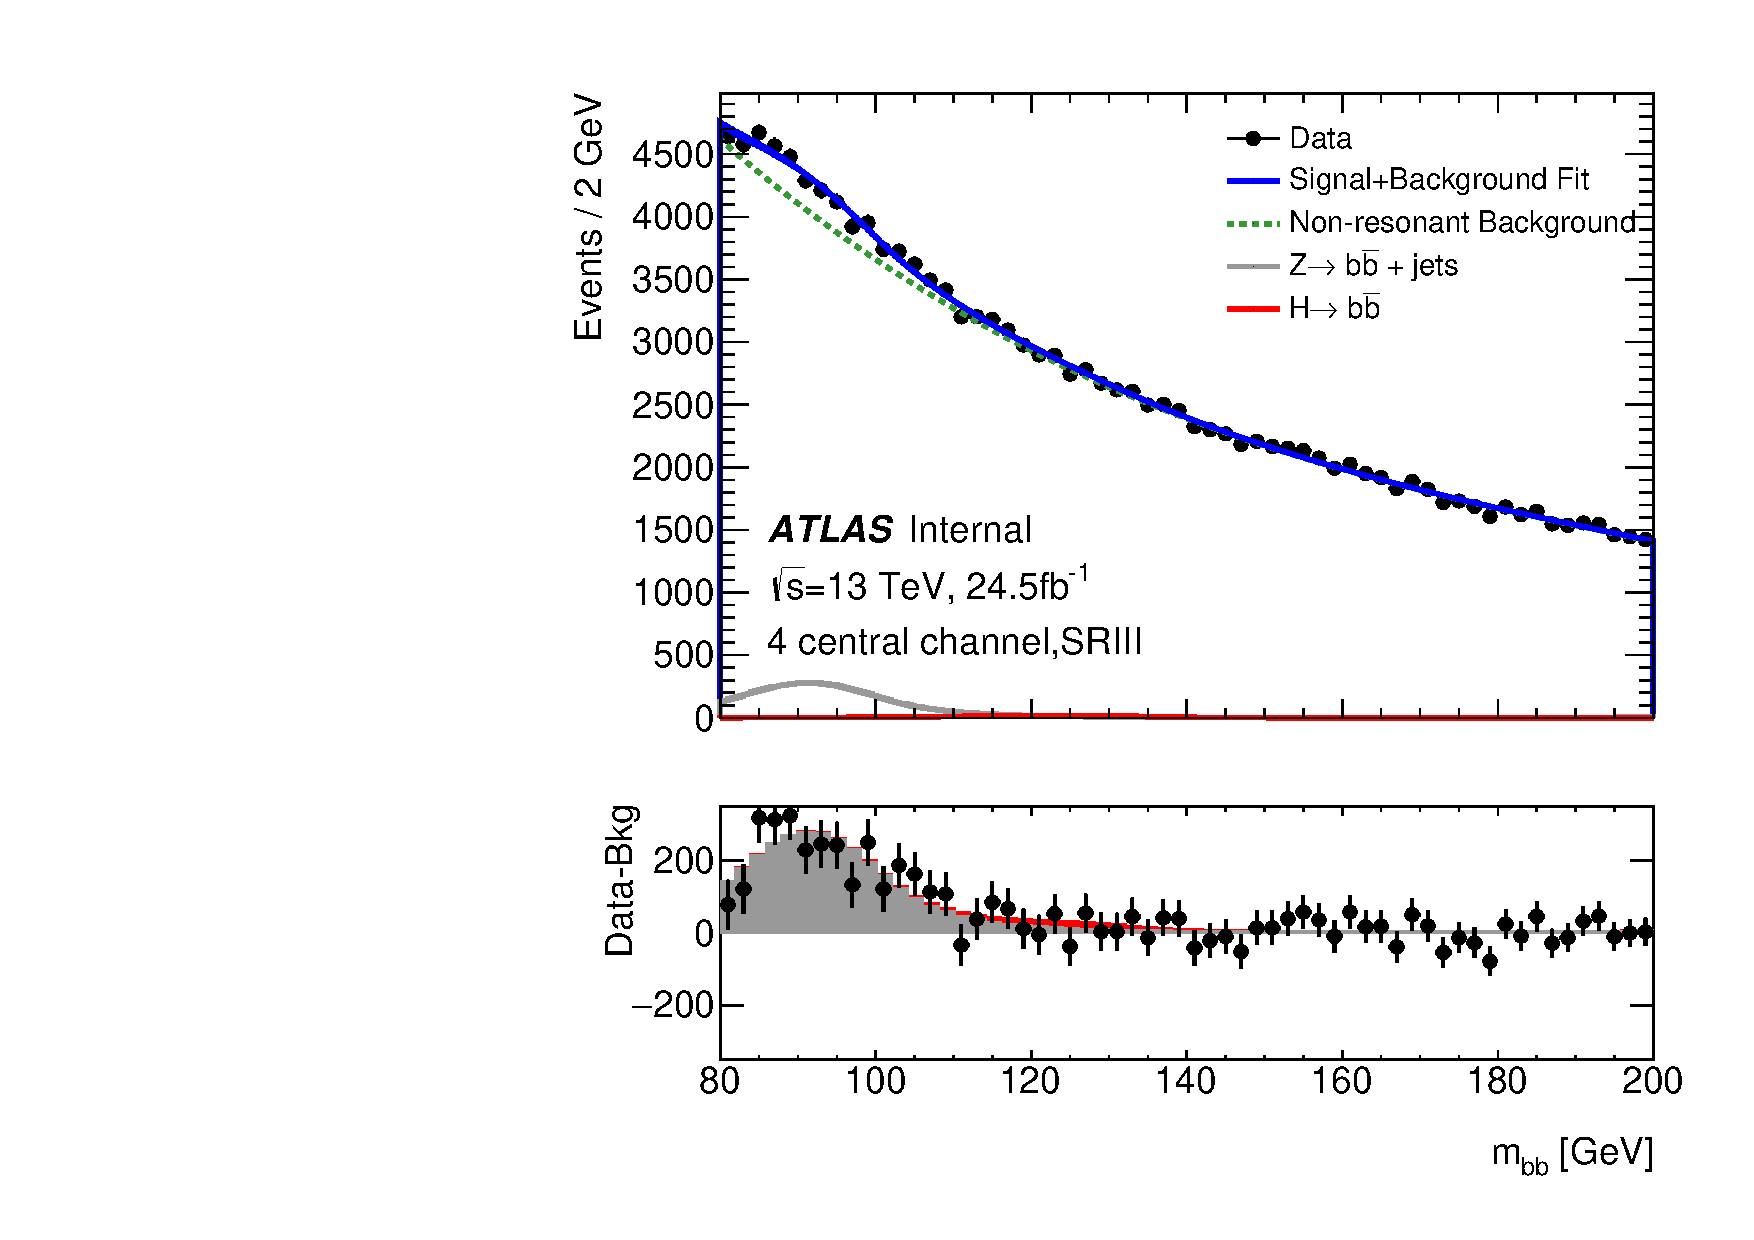
\includegraphics[width=0.48\textwidth]{figures/VBF/unblind_testVBF_ICHEP_4cen_SRIII.pdf}
% 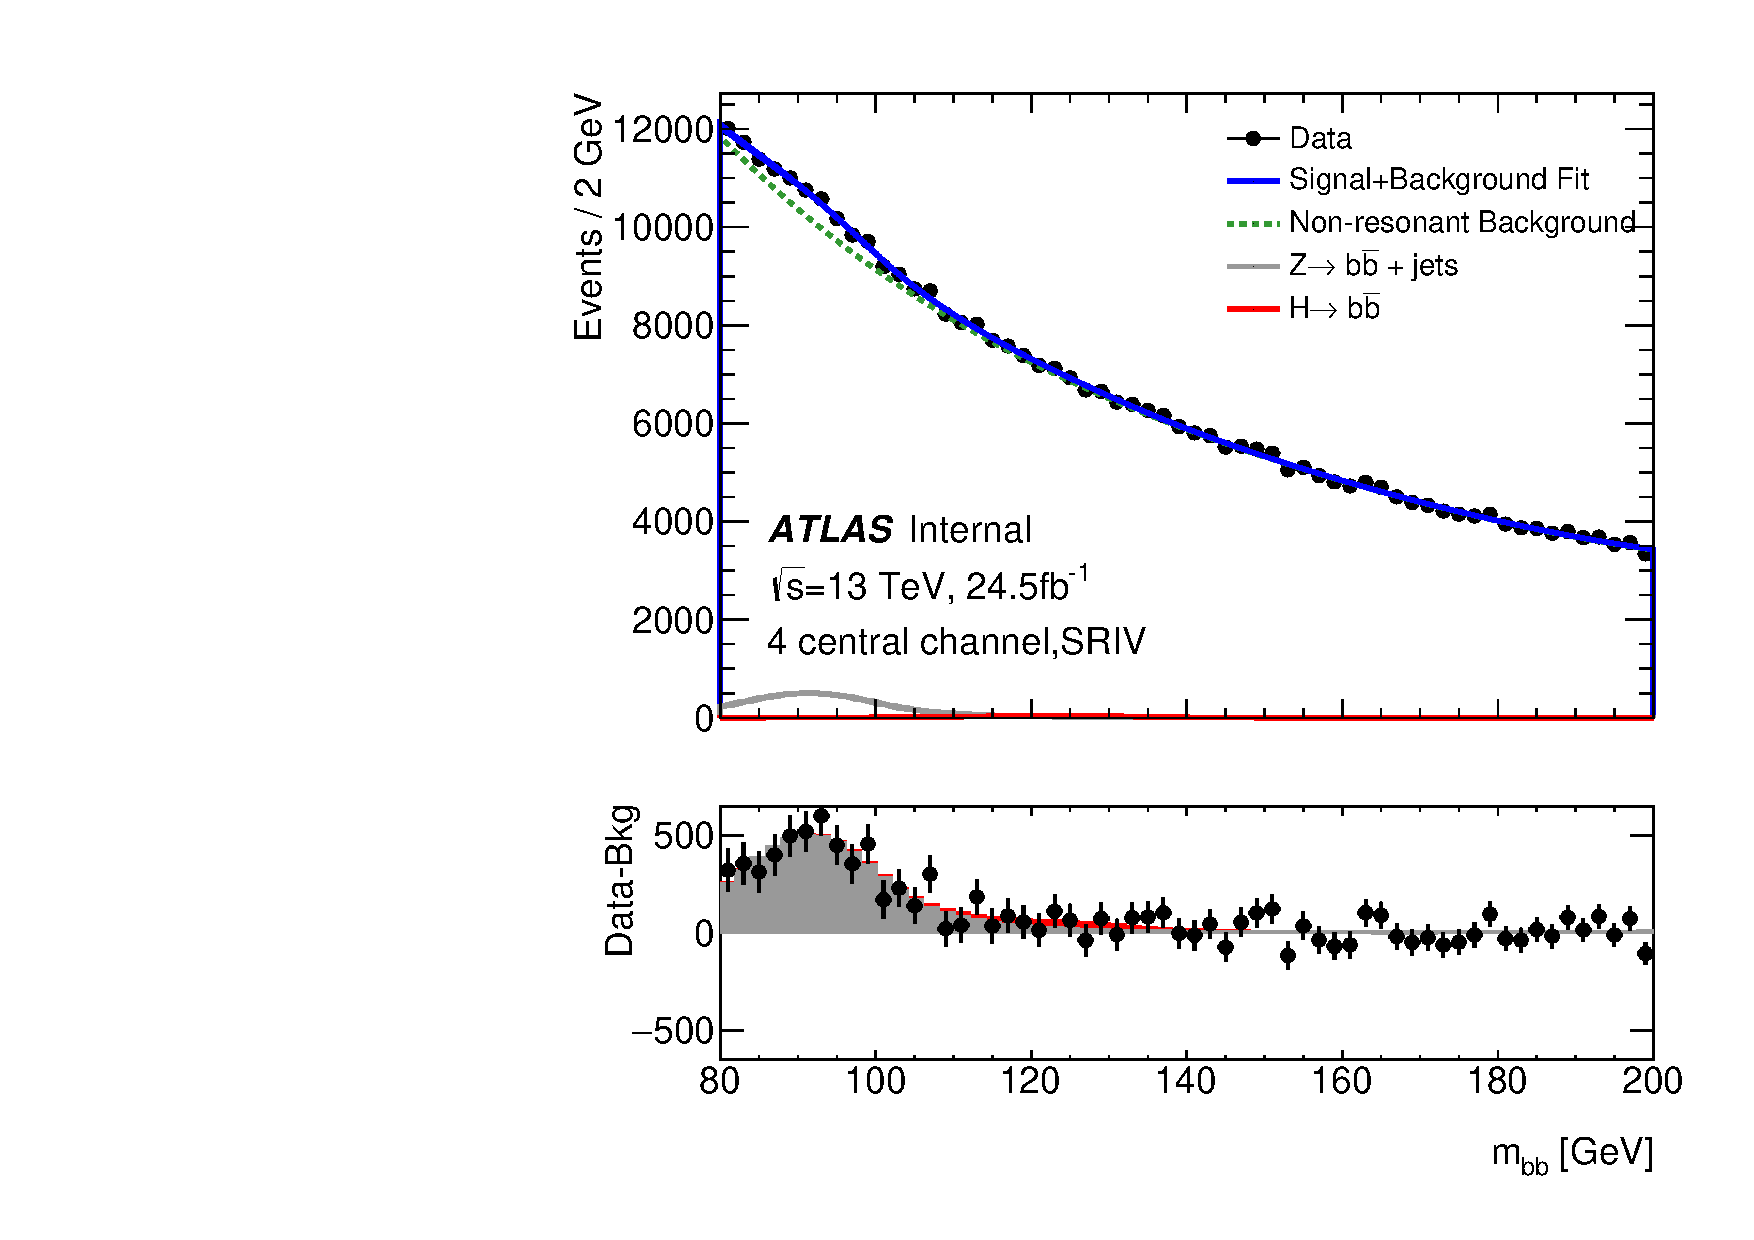
\includegraphics[width=0.48\textwidth]{figures/VBF/unblind_testVBF_ICHEP_4cen_SRIV.pdf}\\
%\caption{Data and fit model comparison for profile likelihood fit in the \fourcentral channel signal regions. The fitted continuum background is shown with at  dashed green line, the fitted $Z$ signal in green, and the fitted Higgs signal in red.  The total fit is displayed as the blue line.  The bottom panels show the residual of the data with respect to the continuum background fit, and the fitted $Z$ signal (grey) and Higgs signal (red) are also displayed.}
%  \label{fig:vbf-higgsfit_4cen}
%\end{figure}


\subsection{Extraction of $\mu_{VBF}$}
\label{sec:vbf-higgsunblindvbf}
A different interpretation of the analysis is the extraction of $\mu_{VBF}$ signal strength.
The fit procedure follows the same way as the extraction of $\mu_{H}$, except we only float
the $VBF$ signal in the fit while fixing the yield of all other Higgs modes, i.e. ggF,
ttH and VH to their Standard Model predictions (with uncertainties applied).
The Asimov fit yields $\mu_{VBF}=1\pm 2.8$. The unblinded value of the VBF Higgs signal
strength is $4.1^{+3.2}_{-2.9}$. The breakdown of the uncertainty
is $\mu_{VBF}=4.1^{+2.8}_{-2.8}\textnormal{(stat)}^{+1.5}_{-0.8}\textnormal{(syst)}$ treating
the NPs for the analytical background parameterization and normalization as well as
the normalization of $Z$ contribution as statistical uncertainty.


\subsubsection{Combination with VBF$+\gamma$ Analysis}
\label{sec:vbf-higgscomb}

The combination of the all-hadronic VBF analysis and the
VBF$+\gamma$ analysis~\cite{vbfplusgammaint} is performed
by a simultaneous likelihood fit to both datasets. The Higgs signal strength is
treated as correlated across all analysis regions,
the $Z$ contributions are extracted as described in the respective analyses.
As described in Section~\ref{sec:vbf-presel}, overlap between the two samples is removed.

The combined fit yields $\mu_H = 2.5^{+1.4}_{-1.3}$ corresponding to an observed significance
of $1.9\sigma$ ($0.8\sigma$ expected). The $VBF$ signal only extraction is also performed combining two analyses similar to \ref{sec:vbf-higgsunblindvbf}. The combined fit yields $\mu_{VBF} =3.0^{+1.7}_{-1.6}$ corresponding to an observed significance of $1.9\sigma$ ($0.7\sigma$ expected). The data and fit model comparisons are shown in Fig.\ref{fig:higgsfit_2cen}\ref{fig:higgsfit_4cen}\ref{fig:mbb_postfit_photon}.

The extractions of $\mu_{H}$ and $\mu_{VBF}$ for separate fits of both all-hadronic and photon analysis and the combination fit are summarized in Fig.\ref{fig:vbf-summary}.


\begin{figure}[htbp]
  \centering
 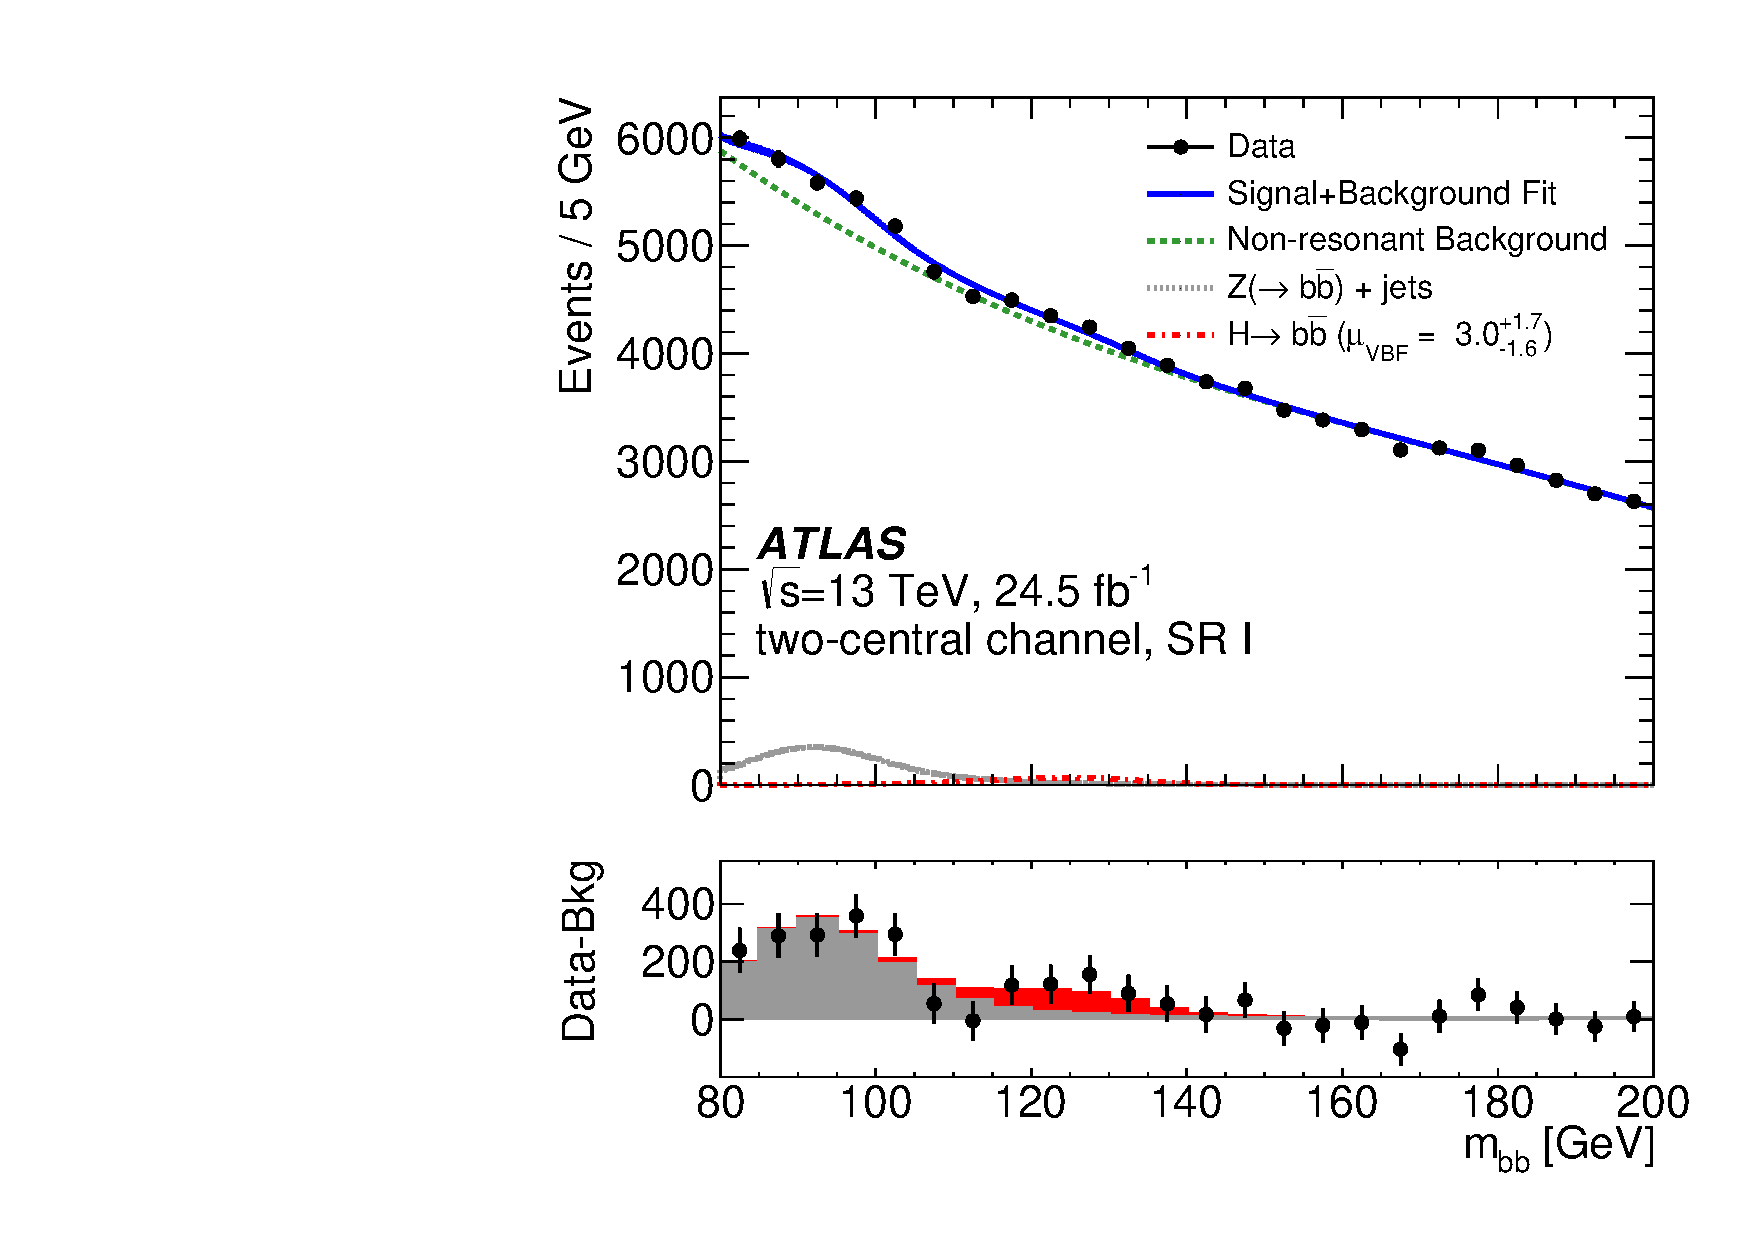
\includegraphics[width=0.48\textwidth]{figures/VBF/comb_vbfonly_testVBF_ICHEP_2cen_SRI_vbfincl.pdf}
 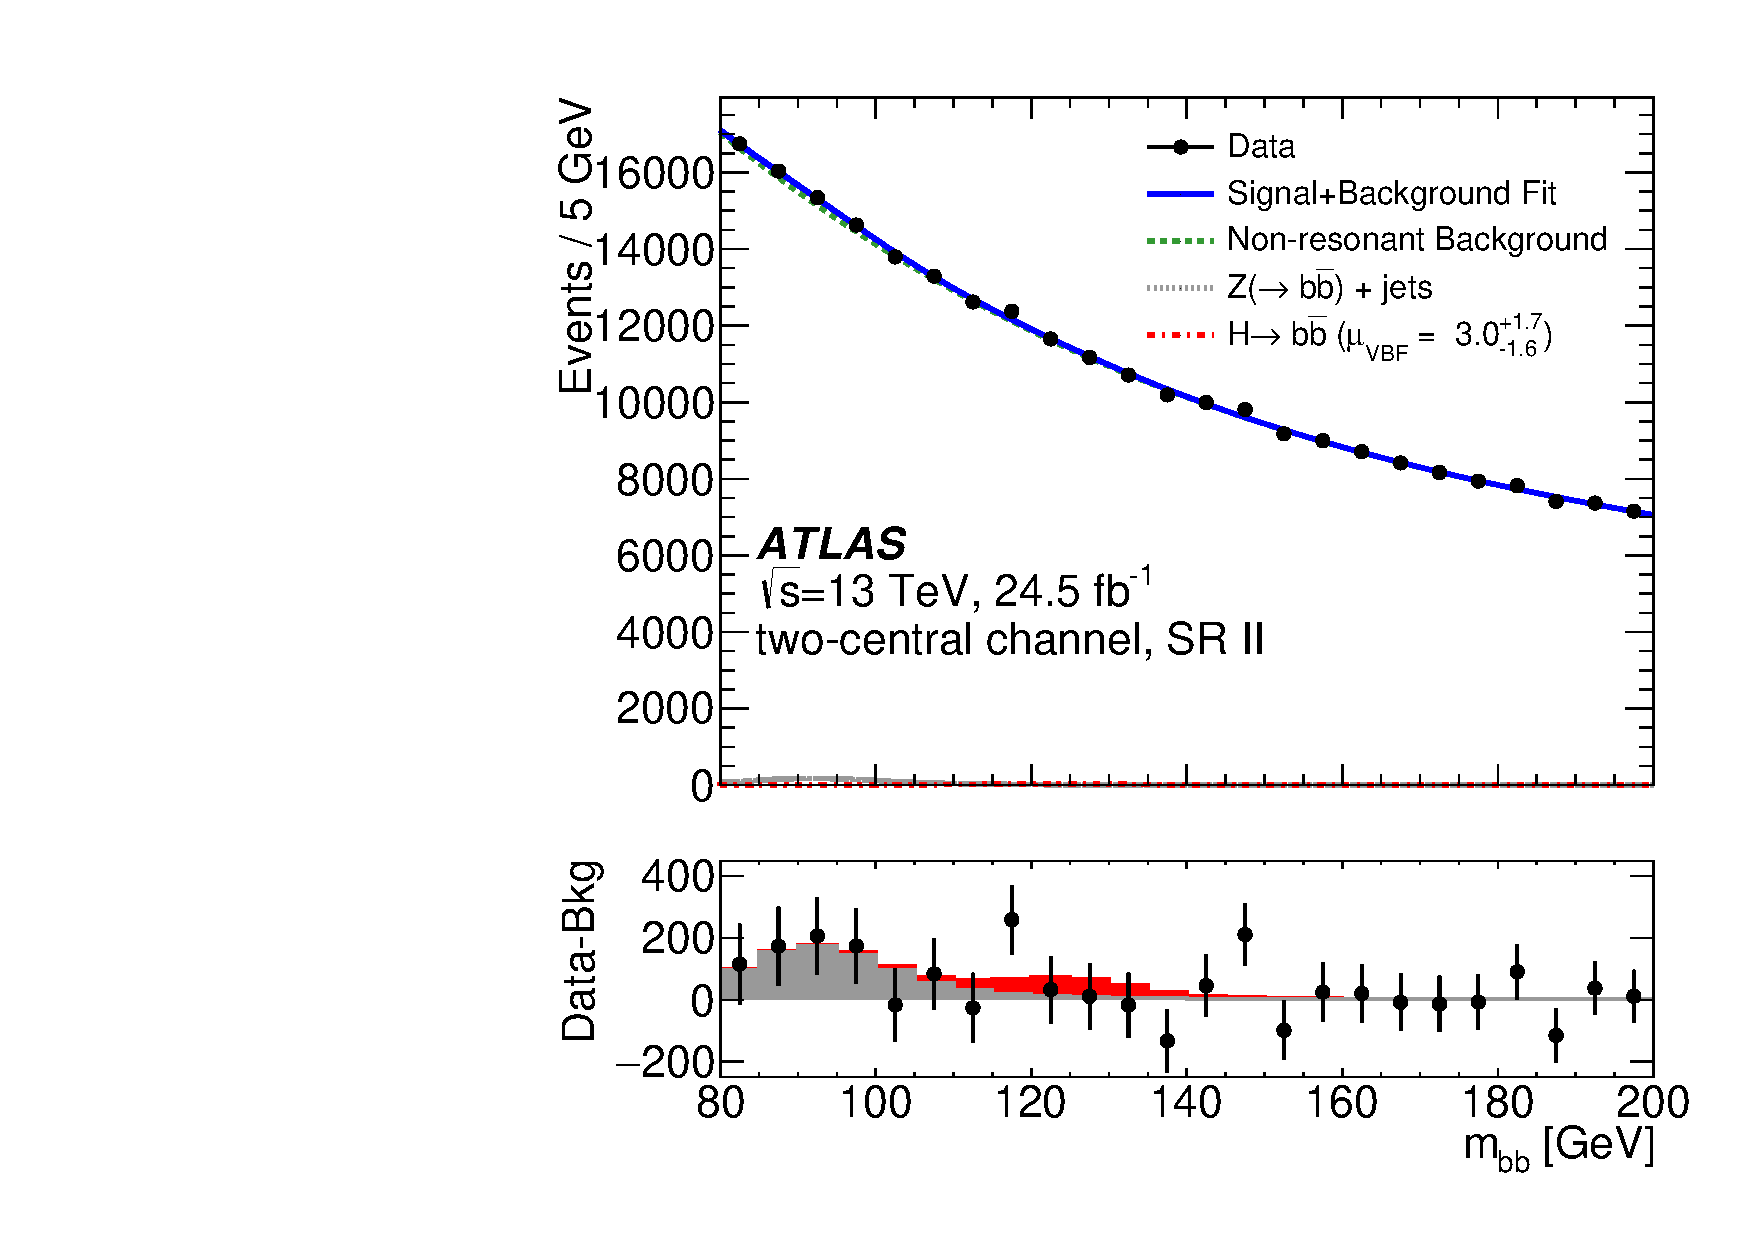
\includegraphics[width=0.48\textwidth]{figures/VBF/comb_vbfonly_testVBF_ICHEP_2cen_SRII_vbfincl.pdf}\\

\caption{Data and fit model comparison for the combined fit of $\mu_{VBF}$ extraction in the \twocentral channel}
  \label{fig:higgsfit_2cen}
\end{figure}

\begin{figure}[htbp]
  \centering
  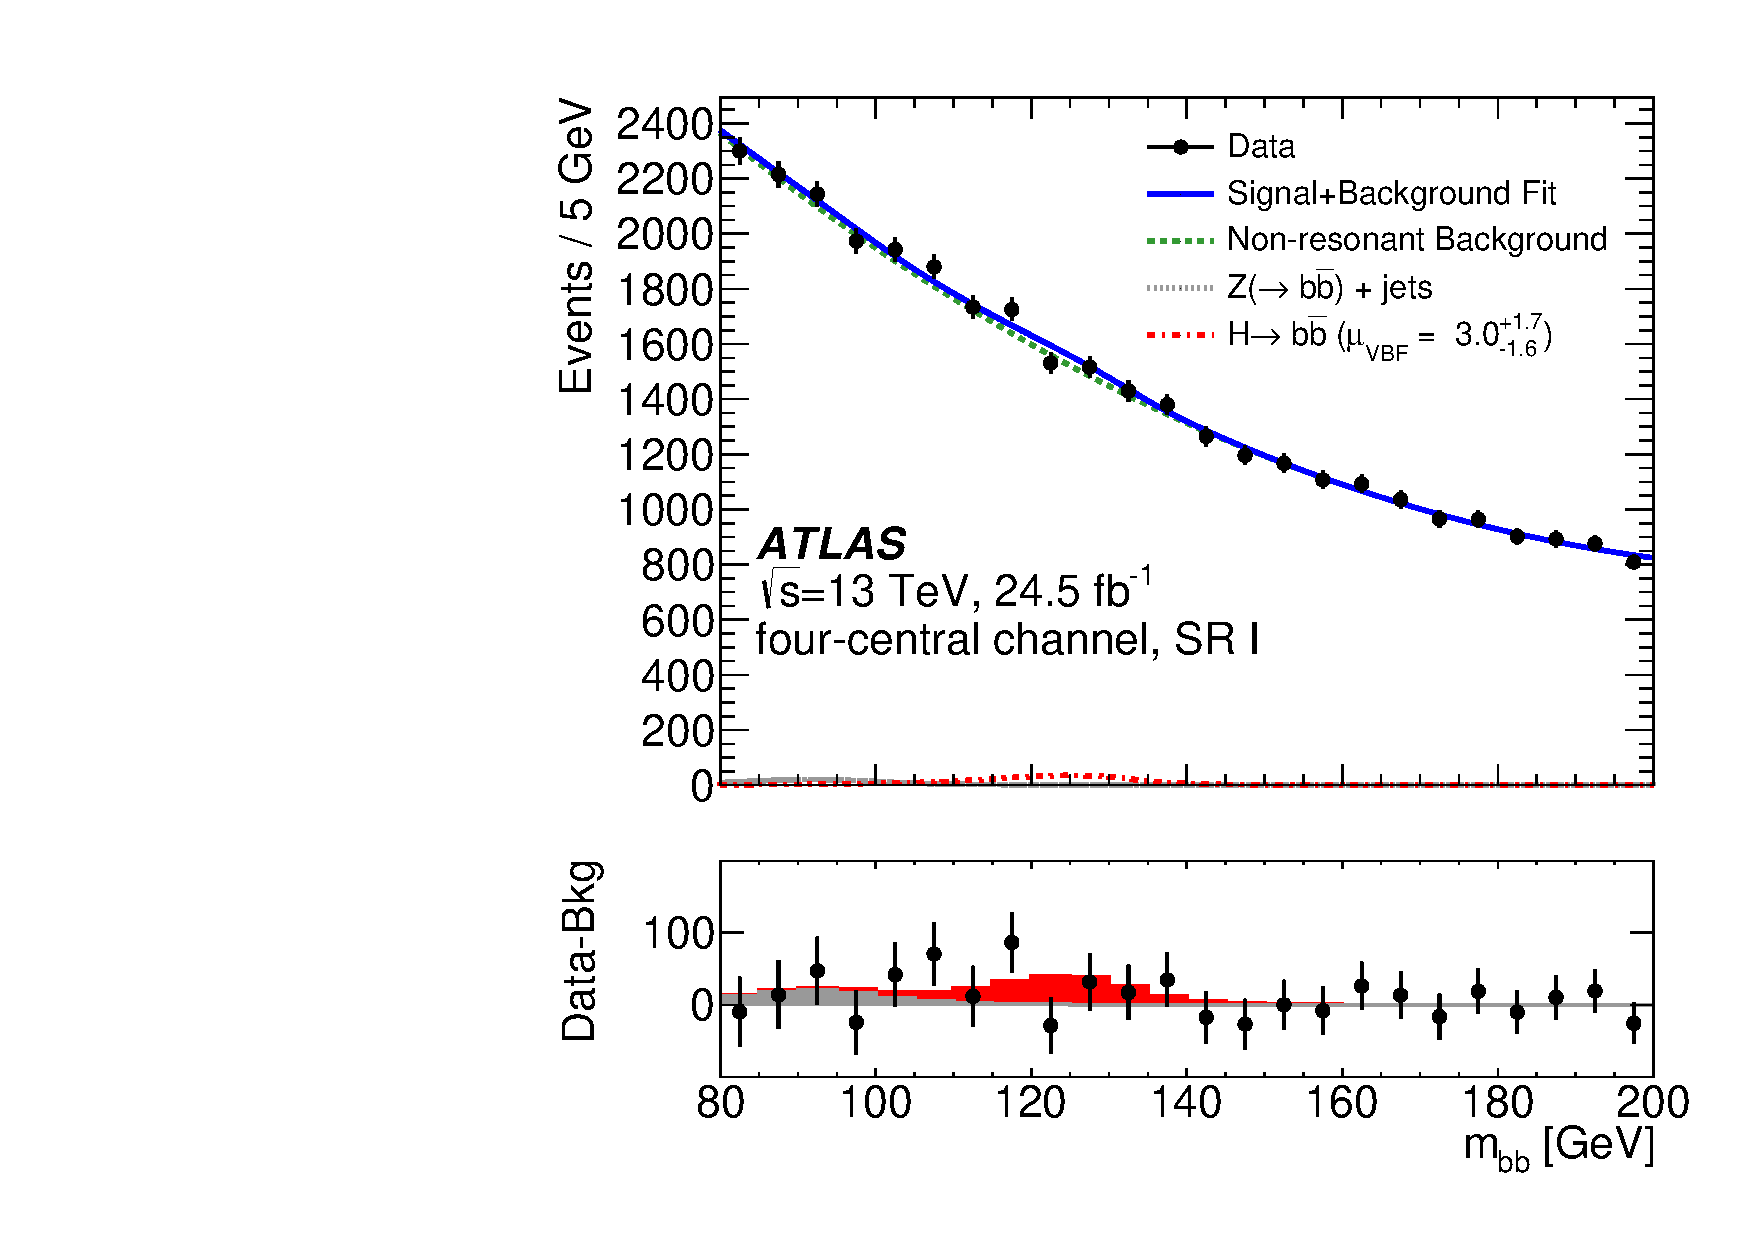
\includegraphics[width=0.48\textwidth]{figures/VBF/comb_vbfonly_testVBF_ICHEP_4cen_SRI_vbfincl.pdf}
 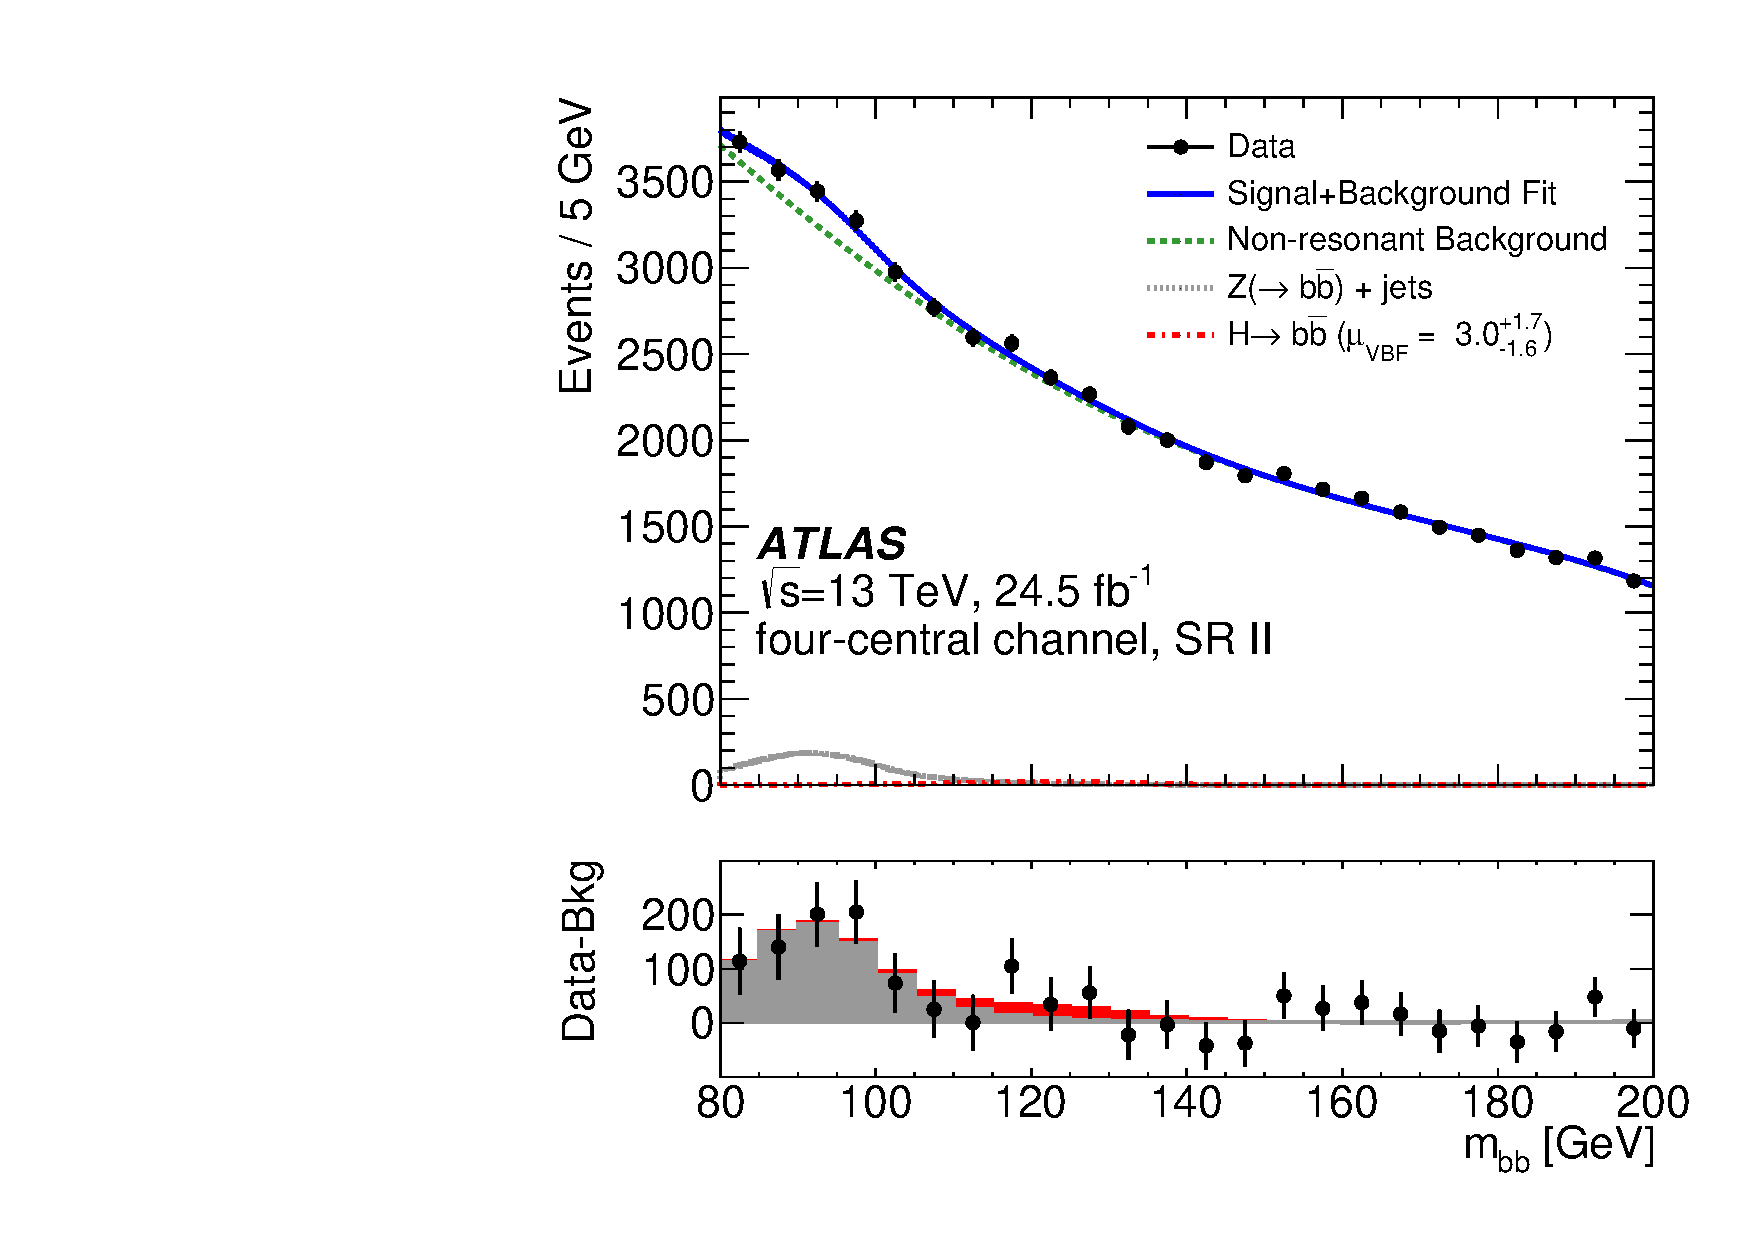
\includegraphics[width=0.48\textwidth]{figures/VBF/comb_vbfonly_testVBF_ICHEP_4cen_SRII_vbfincl.pdf}\\
 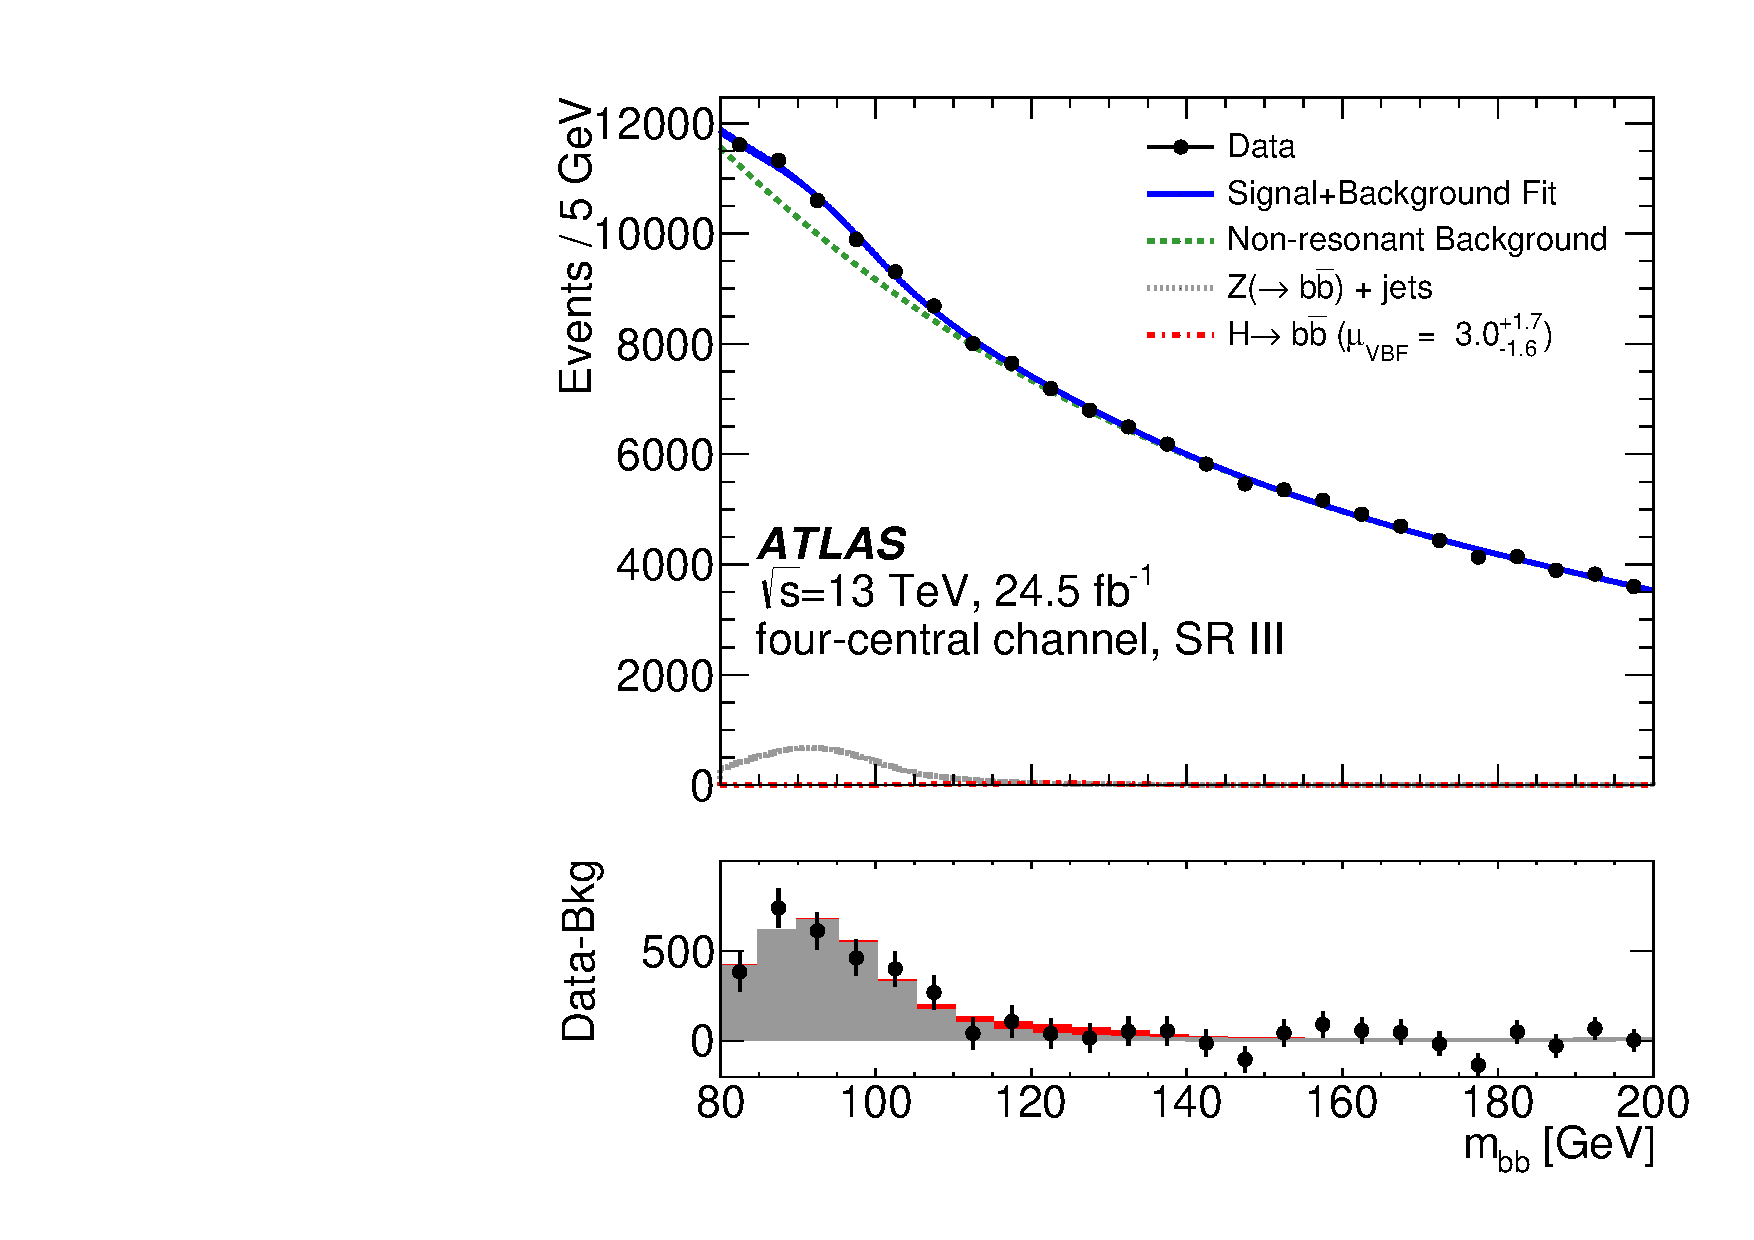
\includegraphics[width=0.48\textwidth]{figures/VBF/comb_vbfonly_testVBF_ICHEP_4cen_SRIII_vbfincl.pdf}
 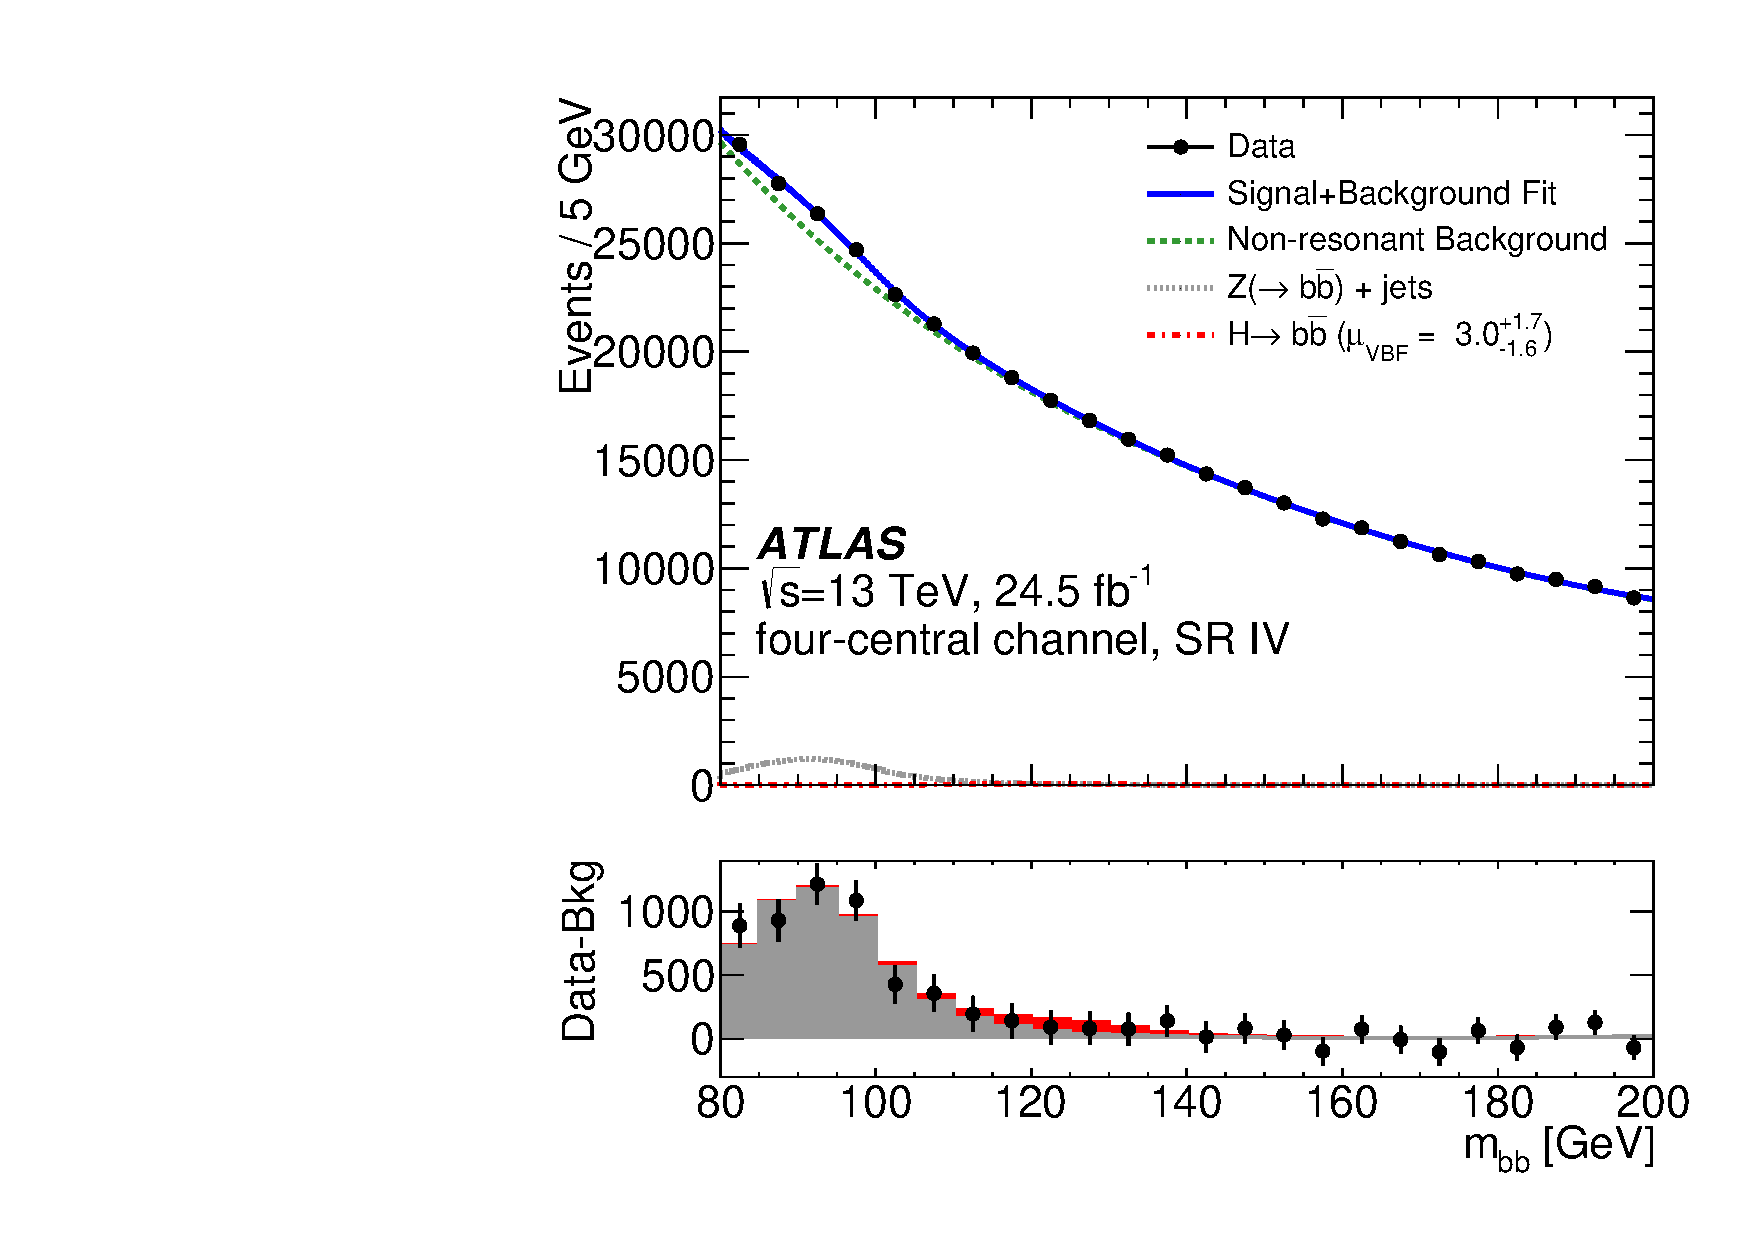
\includegraphics[width=0.48\textwidth]{figures/VBF/comb_vbfonly_testVBF_ICHEP_4cen_SRIV_vbfincl.pdf}\\

\caption{Data and fit model comparison for the combined fit of $\mu_{VBF}$ extraction in the \fourcentral channel}
  \label{fig:higgsfit_4cen}
\end{figure}



\begin{figure}[htbp]
\centering

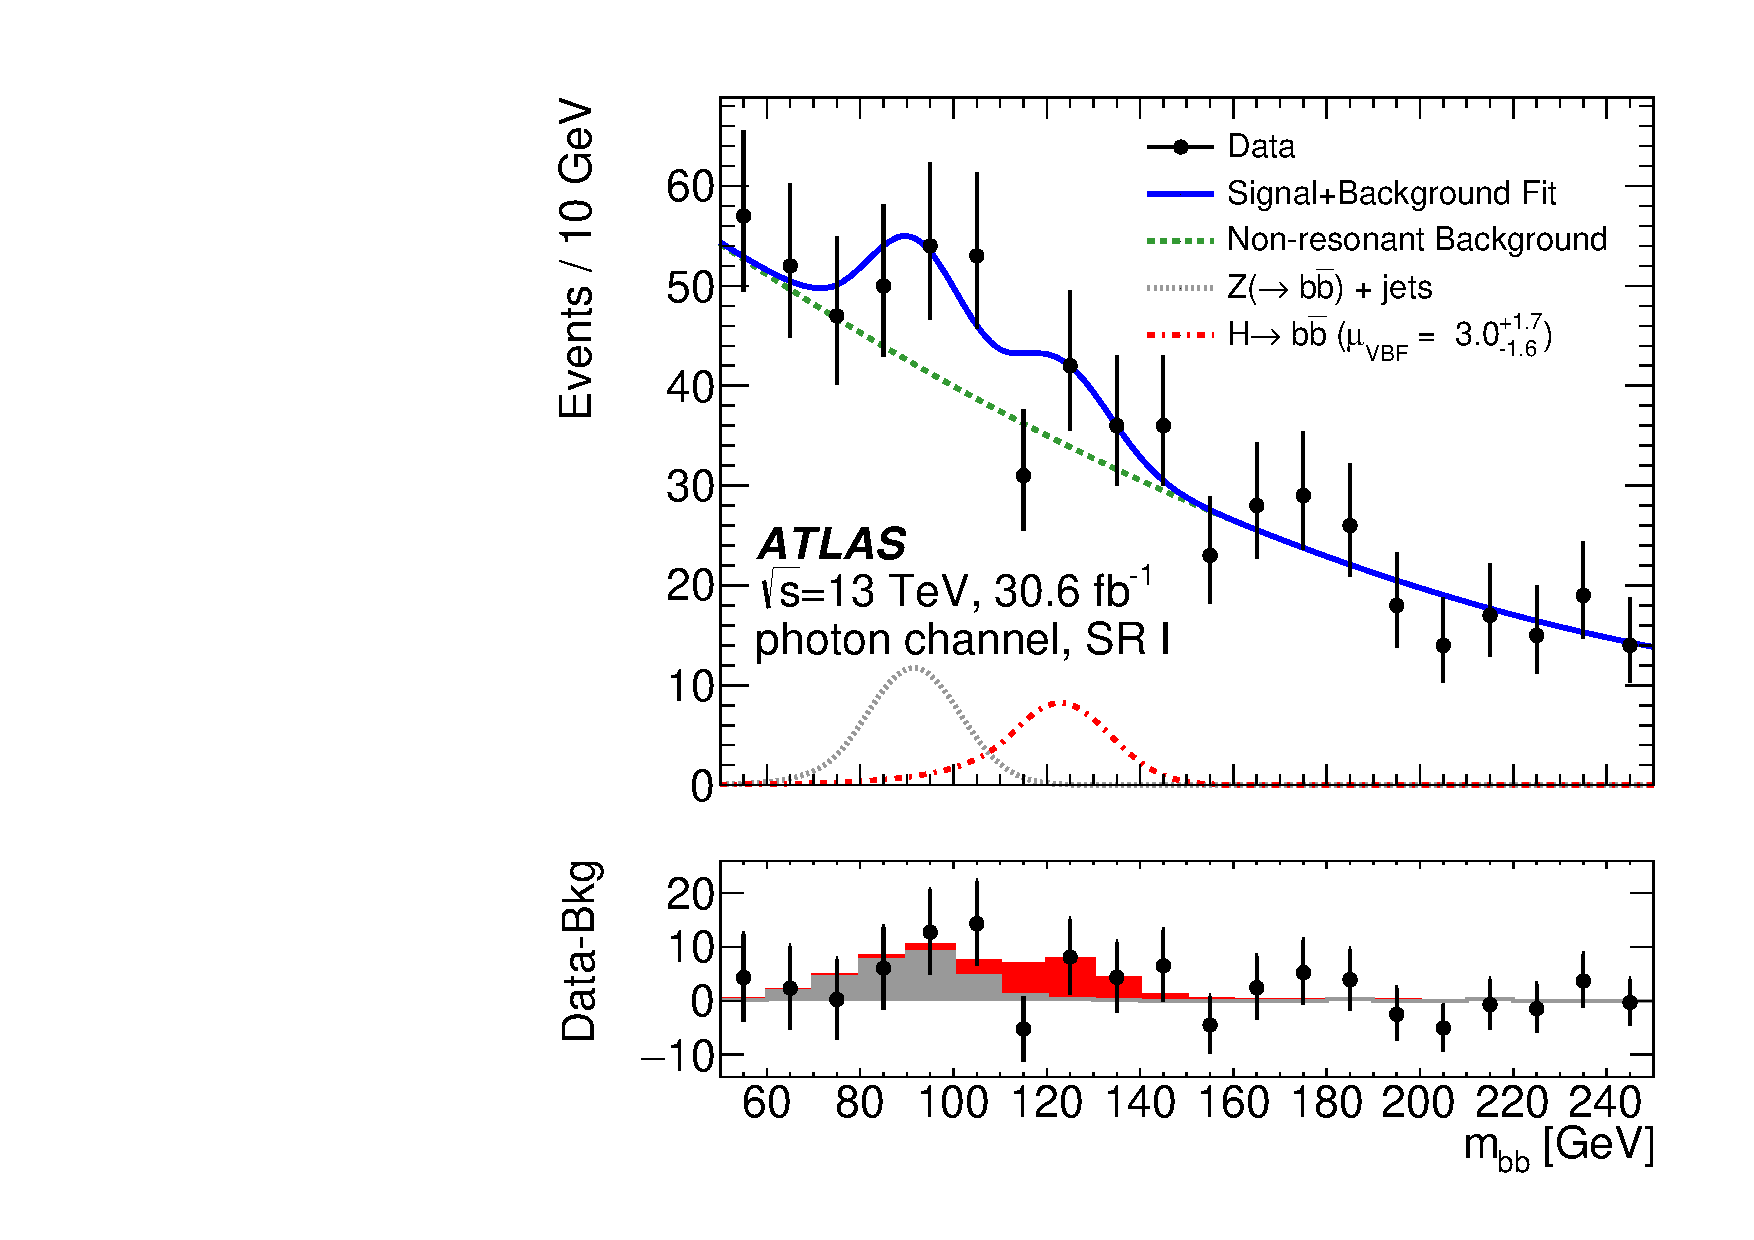
\includegraphics[width=0.48\textwidth]{figures/VBF/comb_vbfonly_testchannel1_vbfg.pdf}
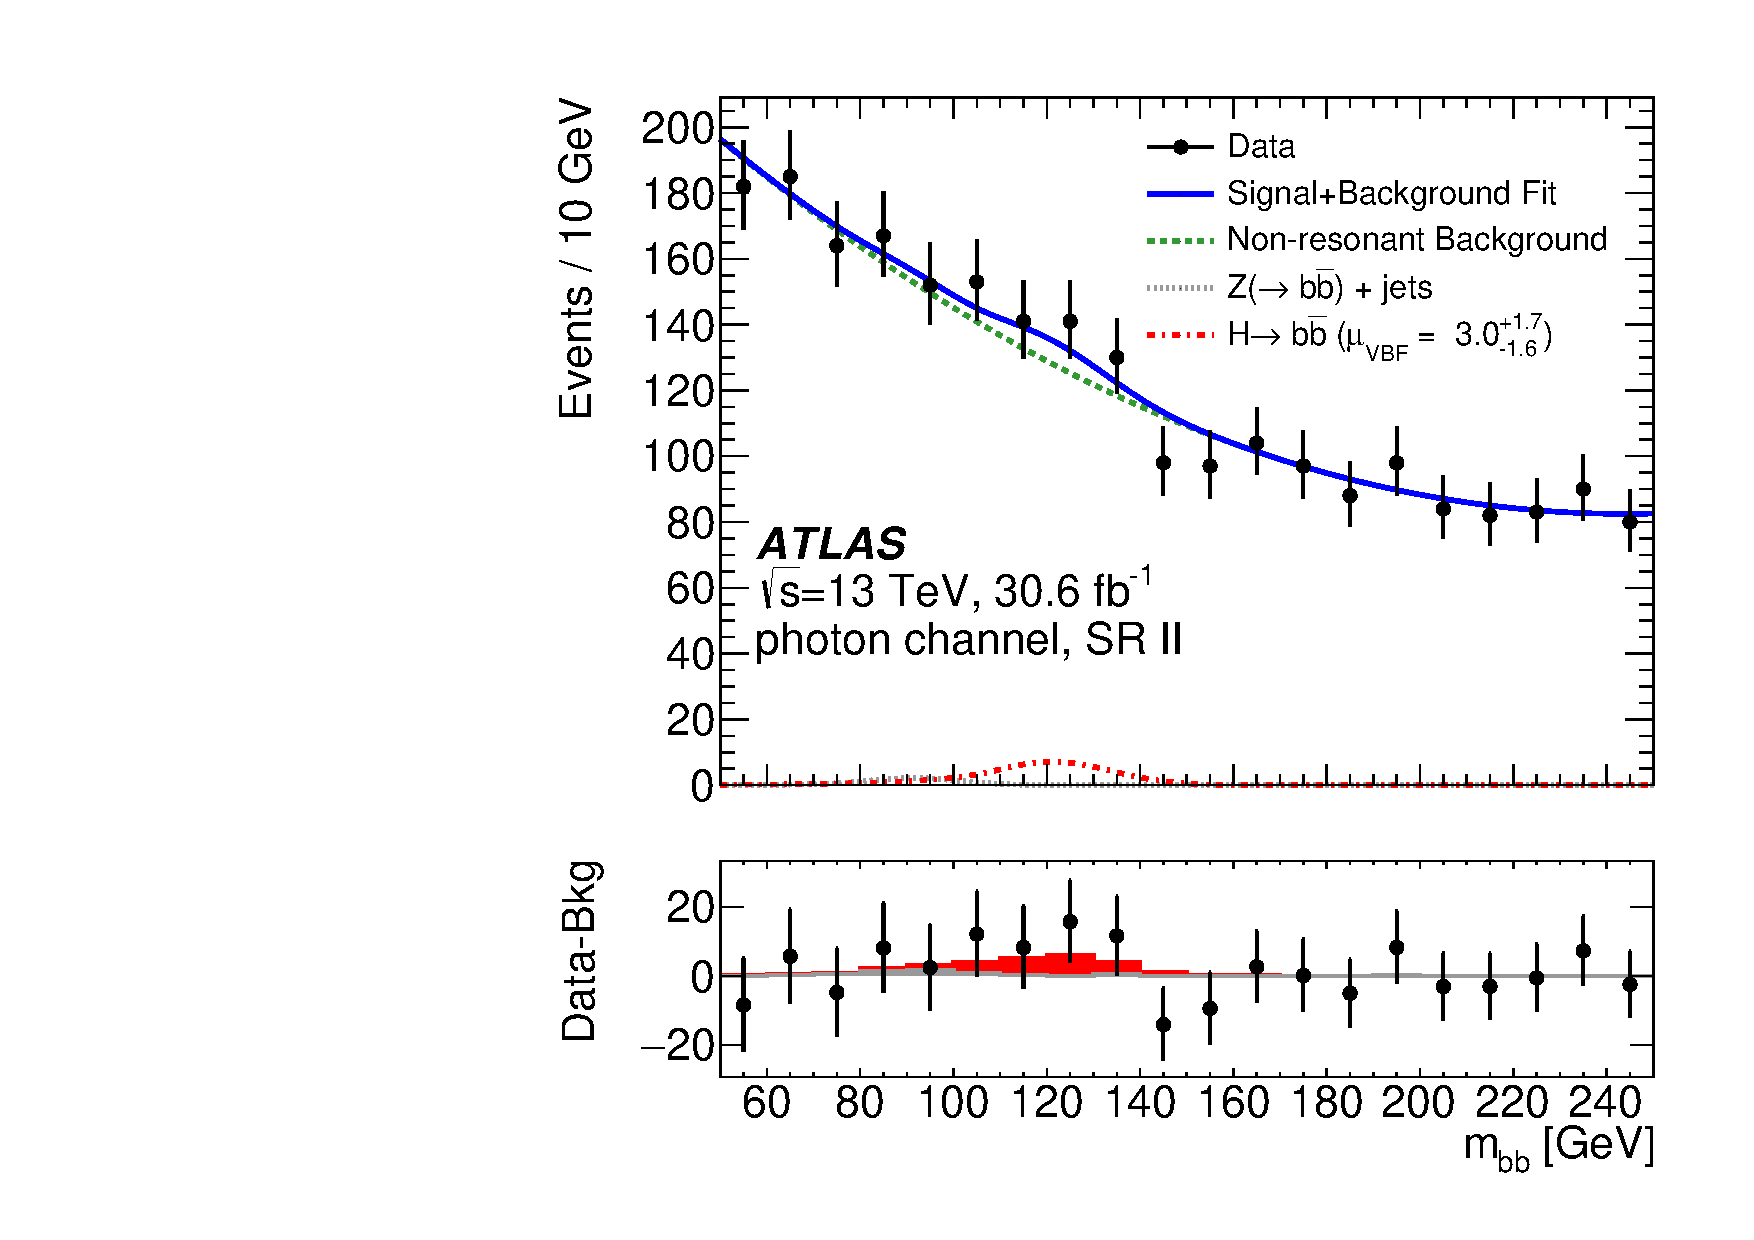
\includegraphics[width=0.48\textwidth]{figures/VBF/comb_vbfonly_testchannel2_vbfg.pdf}
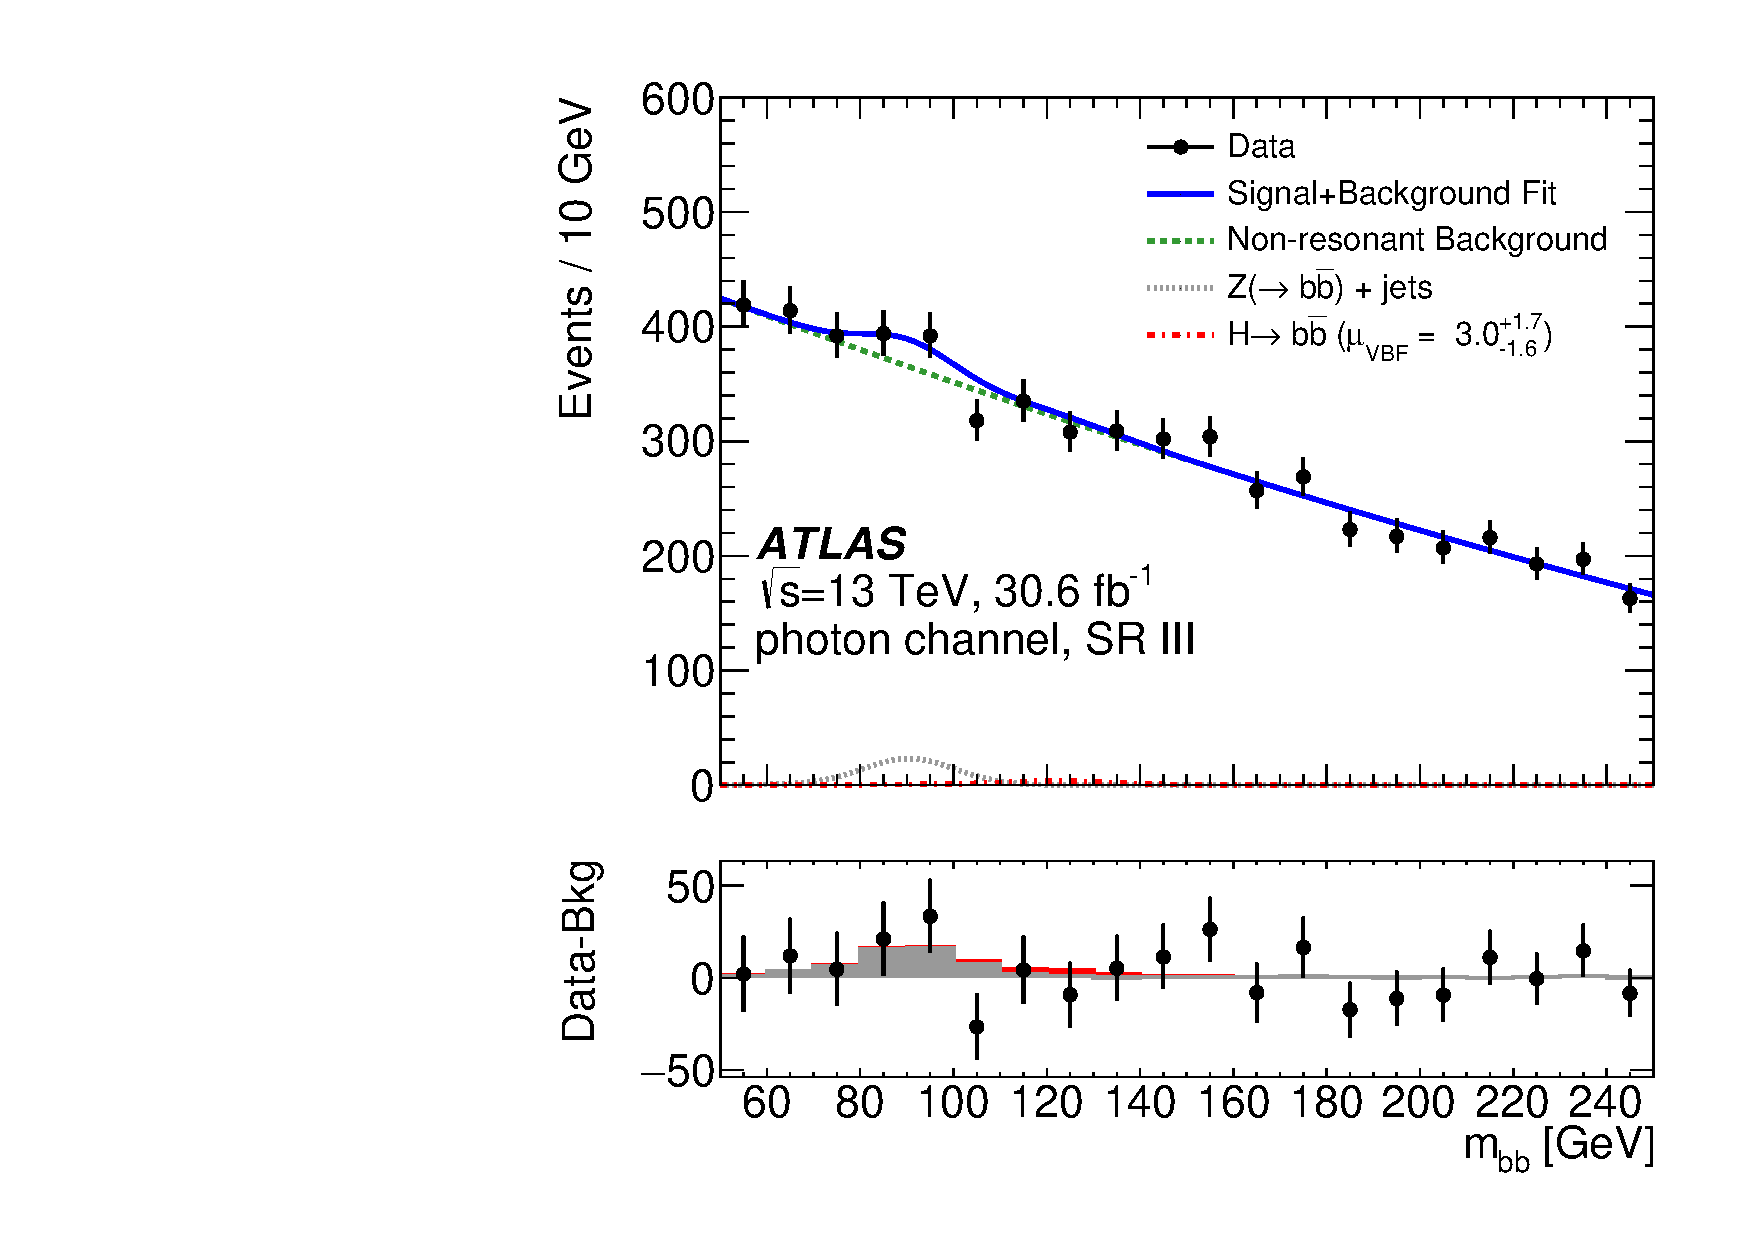
\includegraphics[width=0.48\textwidth]{figures/VBF/comb_vbfonly_testchannel3_vbfg.pdf}
\caption{Data and fit model comparison for the combined fit of $\mu_{VBF}$ extraction in the \textit{photon} channel}
\label{fig:mbb_postfit_photon}
\end{figure}


\begin{figure}[htbp]
  \centering
  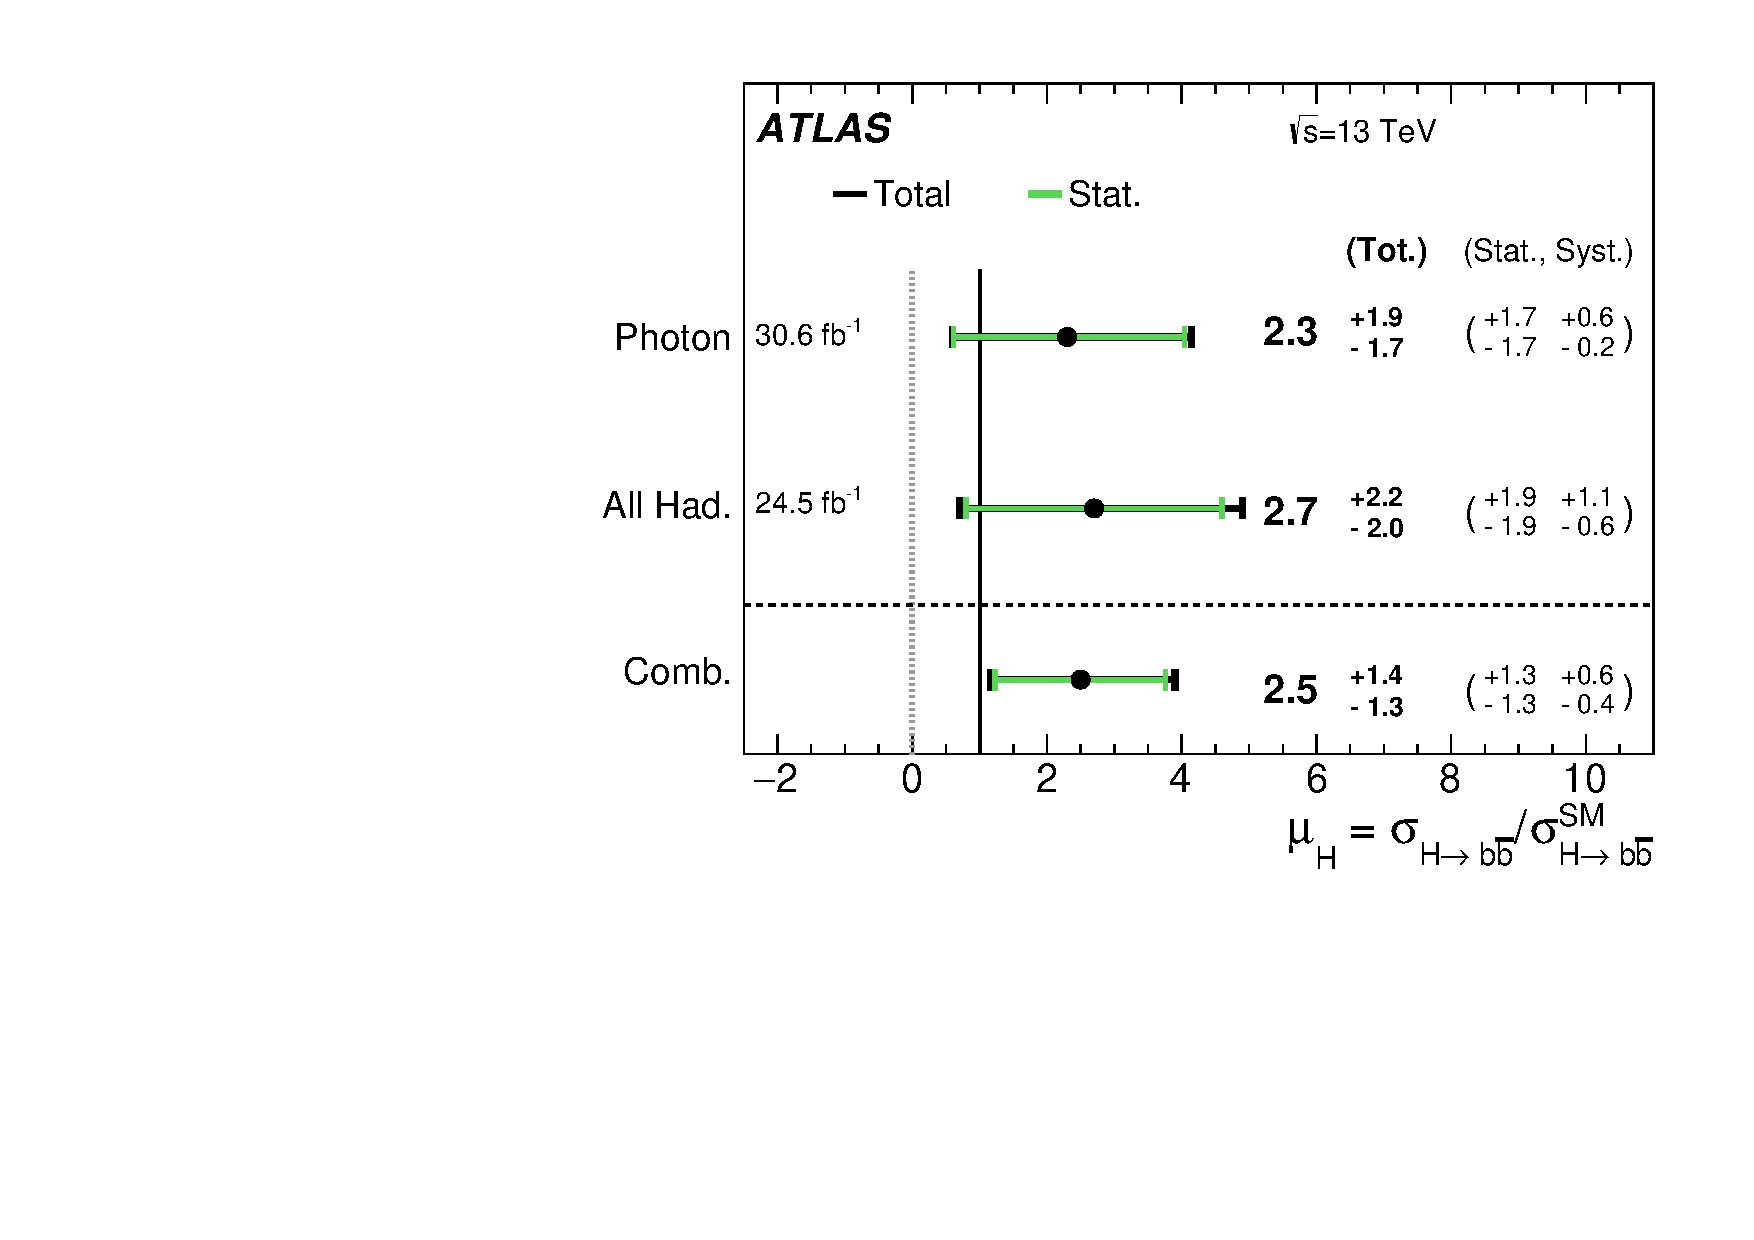
\includegraphics[width=0.49\textwidth]{figures/VBF/Plot_mu_summary_VBF.pdf}
  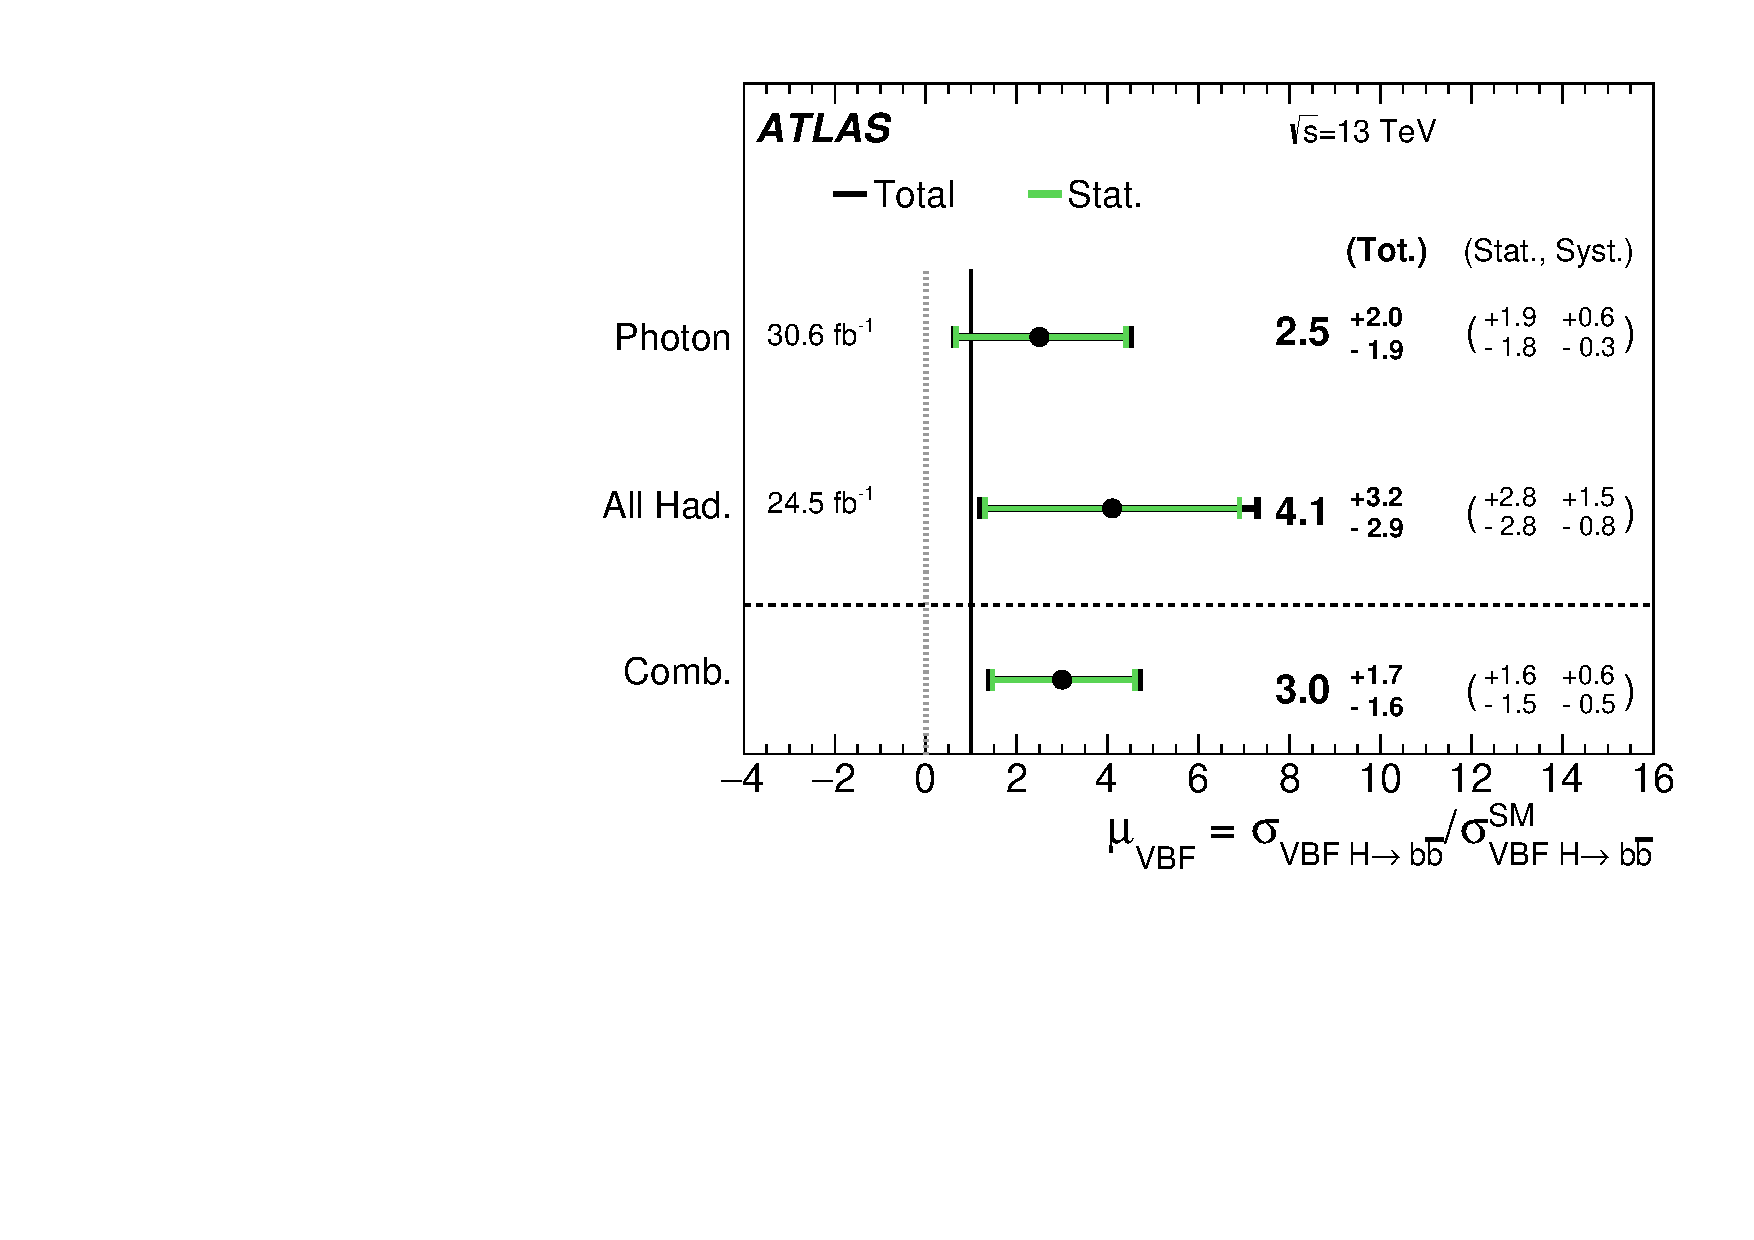
\includegraphics[width=0.49\textwidth]{figures/VBF/Plot_mu_summary_VBFonly.pdf}

\caption{Summary of the extraction of $\mu_{H}$(left) and $\mu_{VBF}$(right) for  \textit{all-hadronic}, \textit{photon} and combination fits.}
  \label{fig:vbf-summary}
\end{figure}



%\begin{figure}[htbp]
%  \centering
% 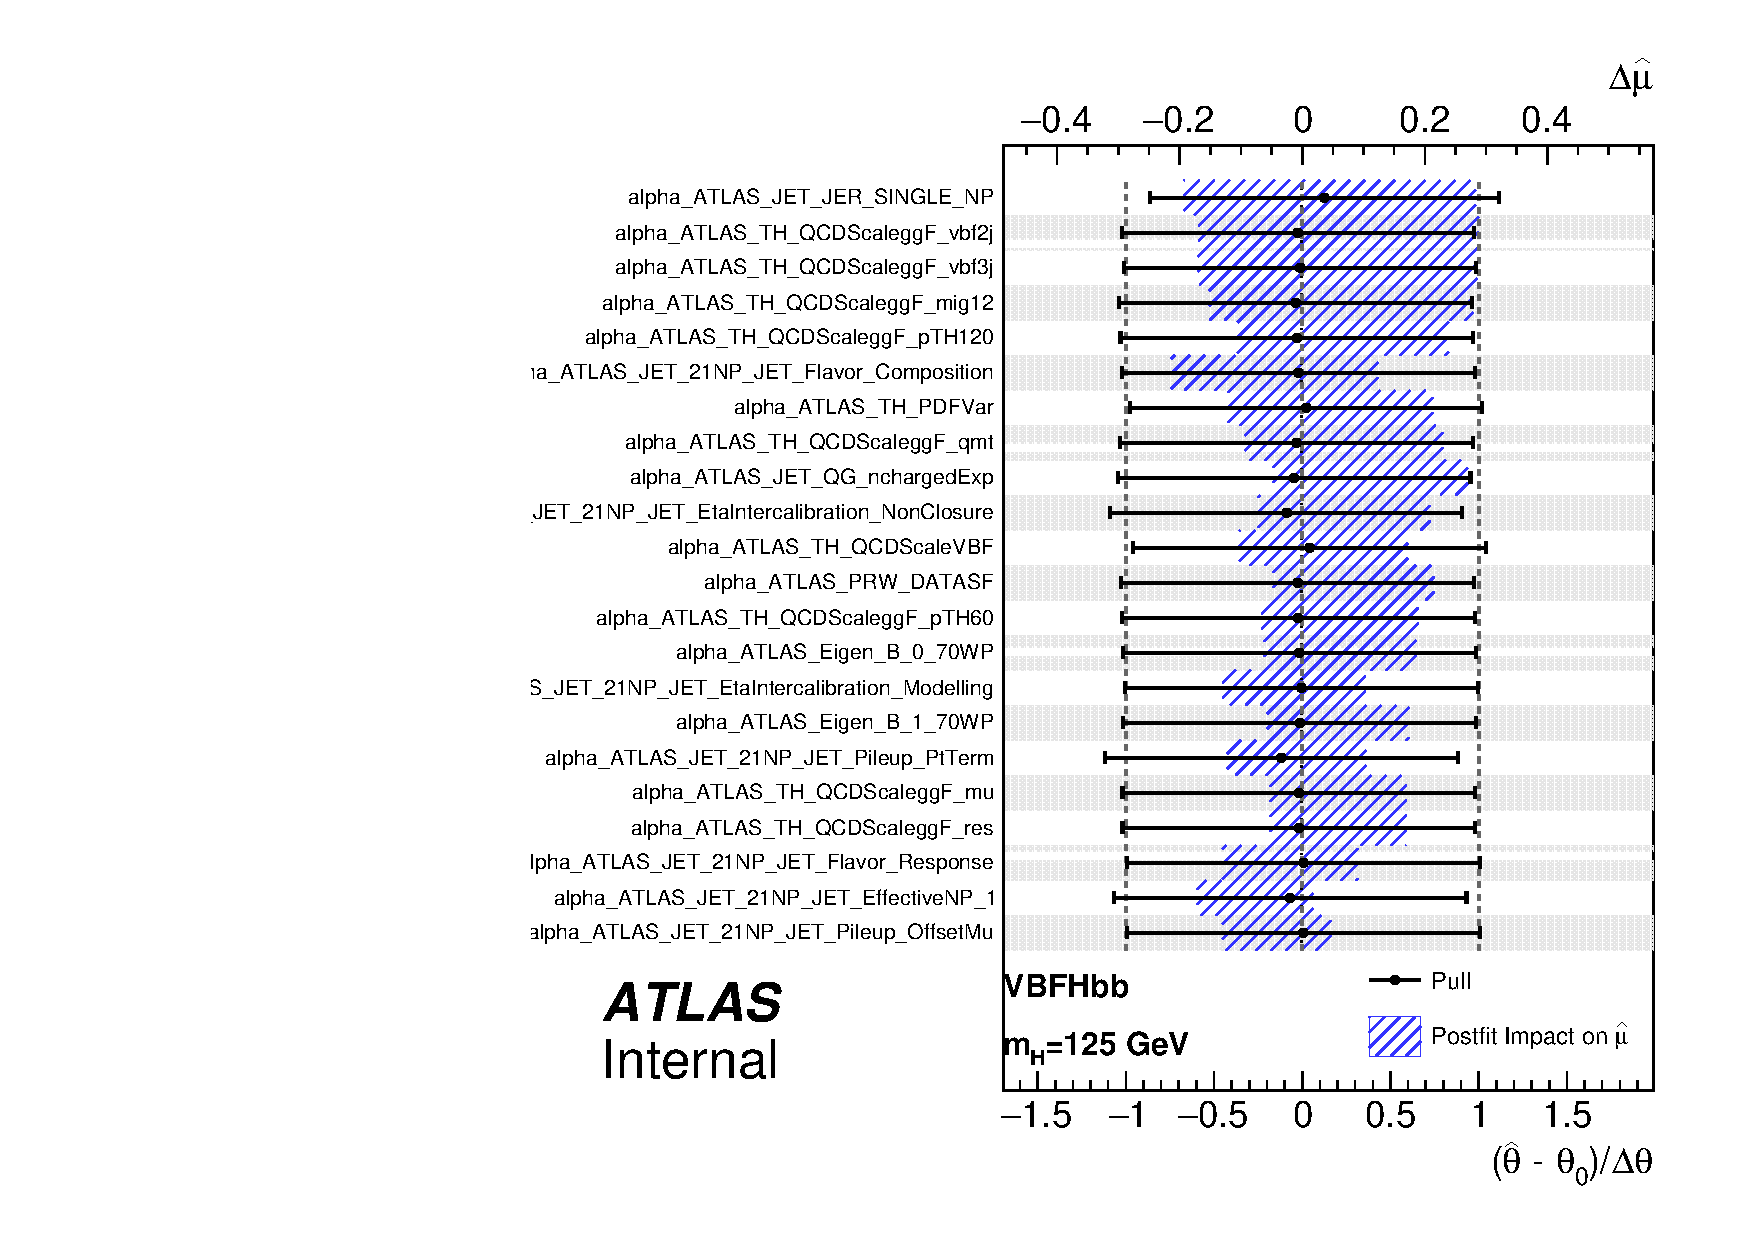
\includegraphics[width=0.8\textwidth]{figures/VBF/VBFHbb_pulls_125.pdf}
% \caption{Nuisance parameter post-fit impact and pulls are plotted for the data fit. Only the constrained NPs are shown. The uncertainties follow the naming defined in Table. \ref{tab:systnames}.}
%  \label{fig:vbf-higgsfitpull}
%\end{figure}


The inclusive and photon analyses apply systematics trimming. The inclusive analyses ignore nuisance parameters with yield impact $<0.5\%$ while the photon analysis ignore systematics with yield impact $<1\%$. Some NPs, for instance the third effective NP of jet energy scale may pass the systematics trimming cut of one analysis but not the other and therefore only show up in the combination fit for one analysis. 

Same set of nuisance parameters of detector related uncertainties including jet energy scale/resolution, luminosity, pile-up reweighting and q/g tagging is used by both analyses and hence treated as correlated.  $b$-tagging related uncertainties are an exception because the operating points are different between the two analyses. The inclusive analysis uses 70\% and 85\% WPs for \twocentral and \fourcentral channels respectively and the VBF$+\gamma$ analysis uses the 77\% WP. We experimented correlating NPs of the $b$-tagging uncertainties with highest impact, e.g. alpha\_FT\_EFF\_Eigen\_B\_0 of different WPs, across the two analyses and observed negligible change in the final result. Therefore the $b$-tagging NPs are left to be un-correlated.

Common terms of theoretical uncertainties including QCD scale of VBF process, parton shower and variation of $ttH$ yield are also correlated as the underlying variations are derived with same approaches. Background systematics such as non-resonant background normalization/parameterization, Z normalization and spurious signals are specific to each analysis and are not correlated.

The combination fit pull for $\mu_H$ is shown in Fig.\ref{fig:vbf-higgsfitpull_combination}. The combination fit pull for $\mu_{VBF}$ is shown in Fig.\ref{fig:vbf-vbffitpull_combination}. One event display for the SRI of the \twocentral channel, the most sensitive BDT region, is shown in Fig.\ref{fig:vbf-evtdisplay}.


%%% no longer needed as VBF inclusive breaks down the QCD scale for VBF and ggF separately:  The inclusive and VBF$+\gamma$ analyses have some overlaps in the treatment of the QCD scale uncertainty although do not use exactly the same procedure therefore, by default, it is treated as uncorrelated.  The VBF$+\gamma$ analysis generates samples at truth level with changes by factors of two in the QCD scale and then does a truth-level calculation of the impact on the acceptance and normalization.  This analysis uses weights generated according to the \textit{WG1 scheme} (see Section~\ref{sec:vbf-syst_model}). Since it is a large systematic uncertainty for both analyses, we also try to correlate this particular nuisance parameter. The combined fit correlating the QCD scale uncertainty yields $\mu_H = 2.40^{+1.37}_{-1.32}$, which has a negligible difference with respect to the uncorrelated treatment. Hence we eventually adopt the result treating QCD scale as un-correlated as it is a more conservative approach. 


\begin{figure}[htbp]
  \centering
 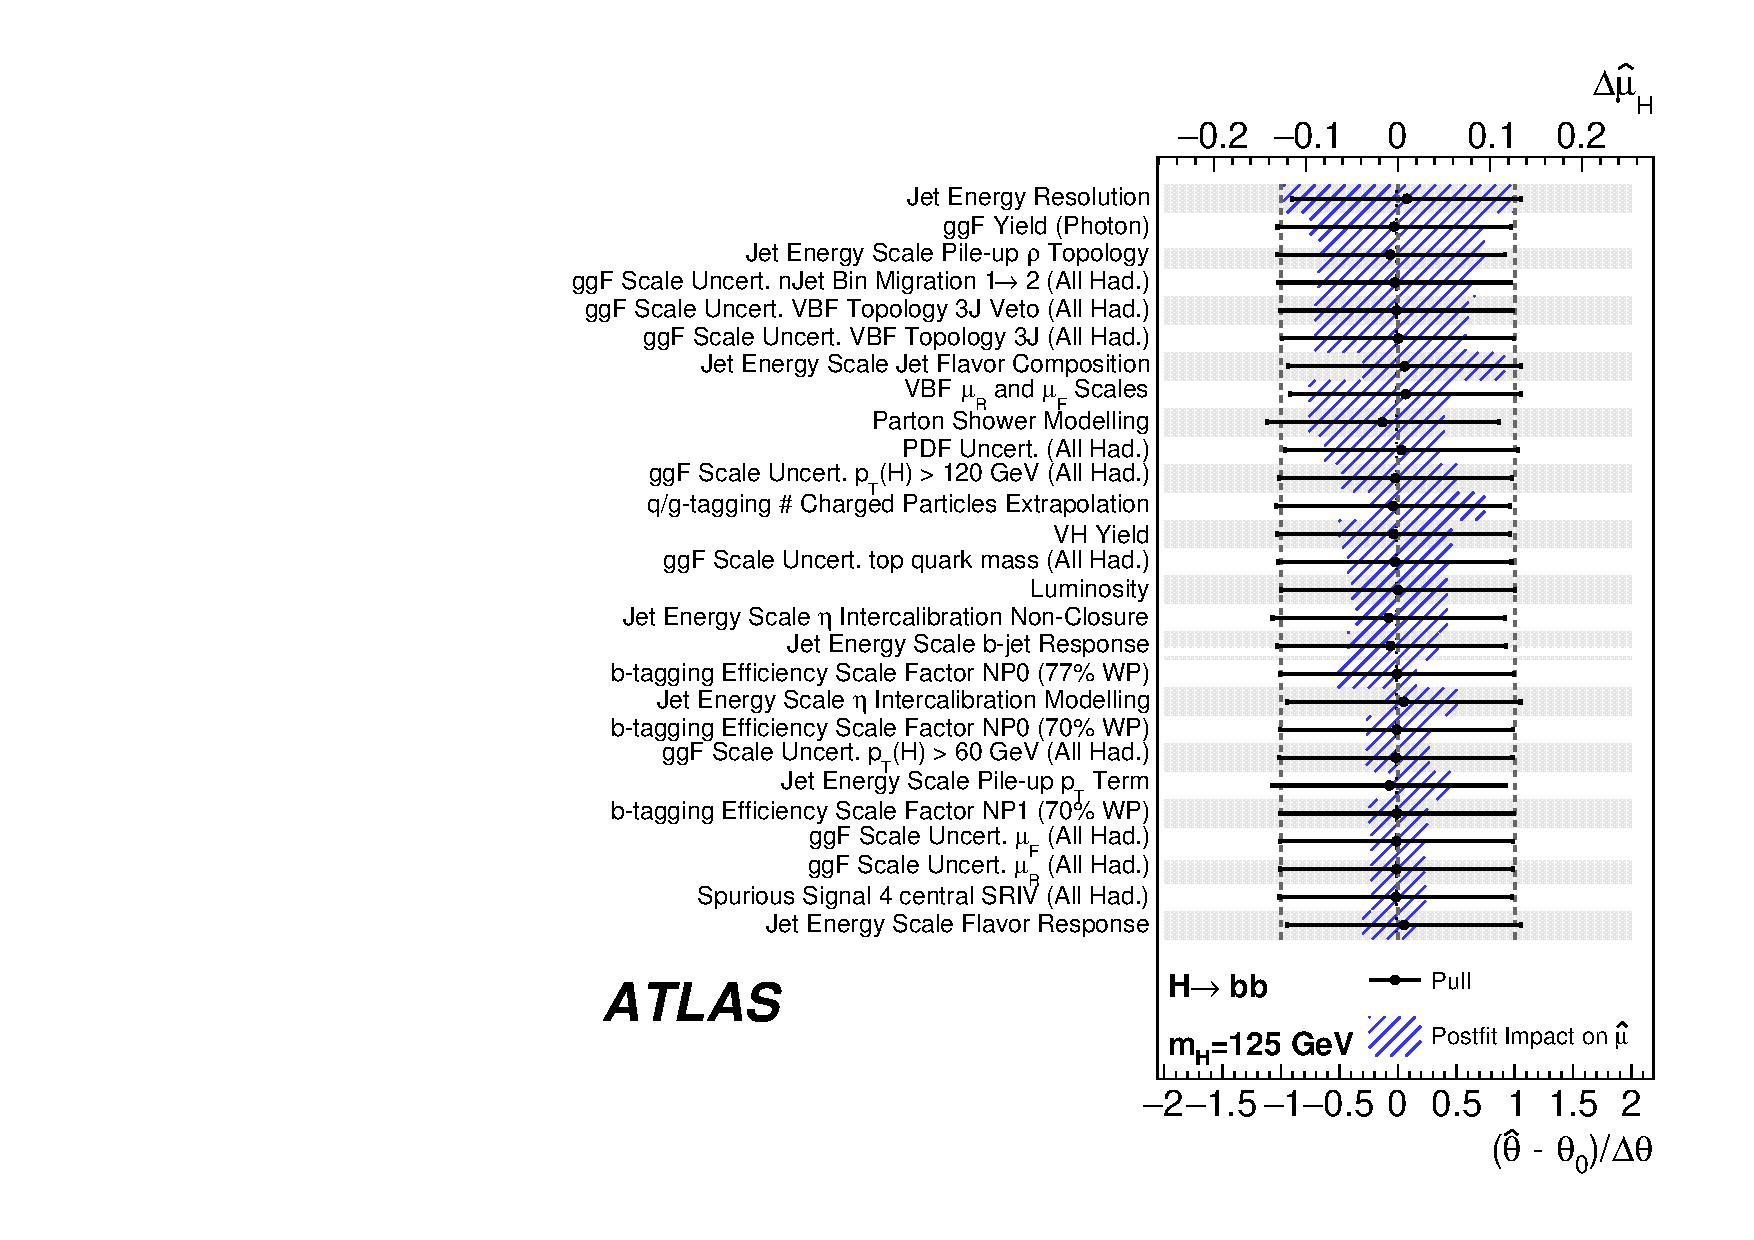
\includegraphics[width=0.8\textwidth]{figures/VBF/VBFHbb_Combined_pulls_125.pdf}
\caption{Data fit pulls for nuisance parameters with a post-fit impact $> 2$ \% for $\mu_H$ combining VBF inclusive and VBF$+\gamma$ analyses.}
  \label{fig:vbf-higgsfitpull_combination}
\end{figure}

\begin{figure}[htbp]
  \centering
 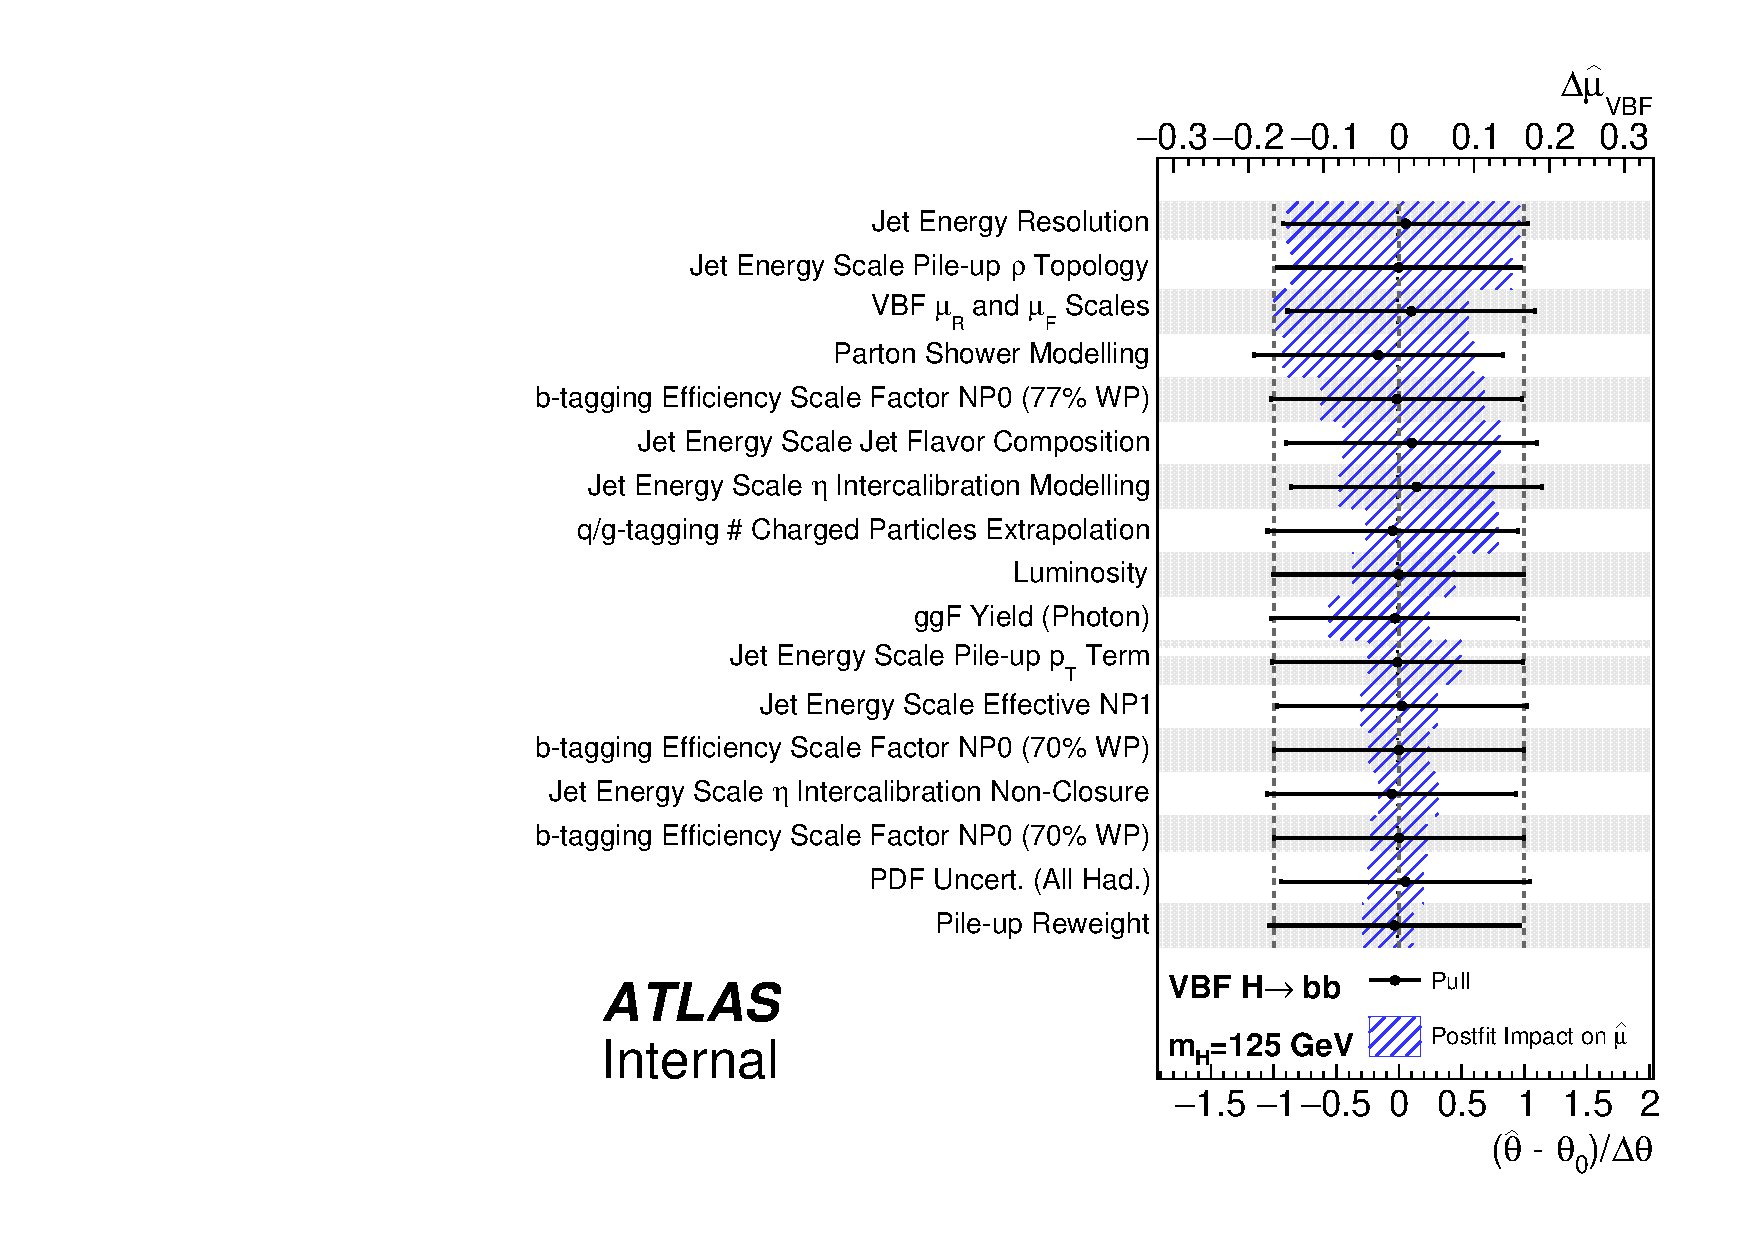
\includegraphics[width=0.8\textwidth]{figures/VBF/VBFHbb_Combined_vbfonly_pulls_125.pdf}
\caption{Data fit pulls for nuisance parameters with a post-fit impact $> 2$ \% for $\mu_{VBF}$ combining VBF inclusive and VBF$+\gamma$ analyses.}
  \label{fig:vbf-vbffitpull_combination}
\end{figure}


\begin{figure}[htbp]
  \centering
 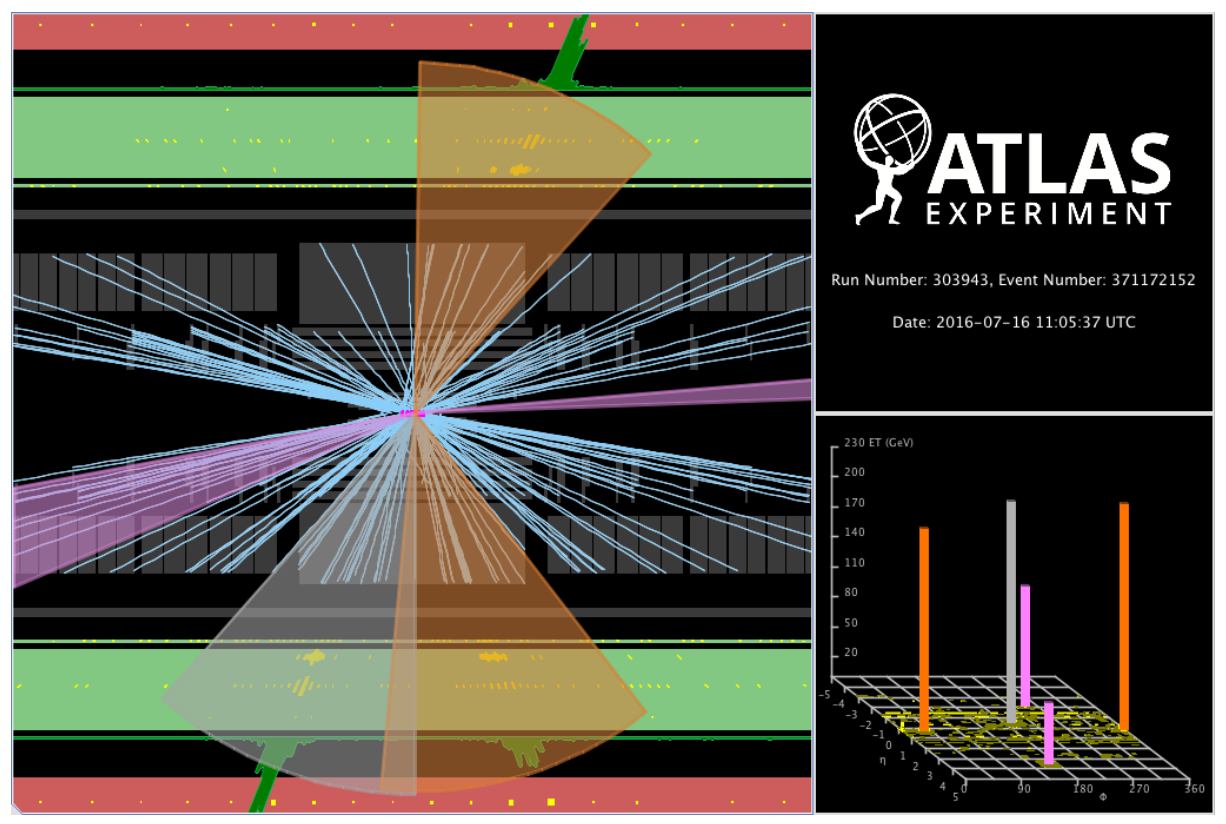
\includegraphics[width=0.8\textwidth]{figures/VBF/EvtDisplay2cen}
\caption{Event display of a \twocentral candidate event in SR I of the with \Mbb = 147 GeV. The cones representing the jets are colored magenta for the forward jets and orange for the b-tagged jets. The transverse momenta of the leading forward jet and sub-leading forward jet are 130.5 GeV and 82.0 GeV respectively. The pseudorapidity of the leading forward jet and sub-leading forward jet are -2.0 and 3.6 respectively}
  \label{fig:vbf-evtdisplay}
\end{figure}


